\section{実験}

雨が降るシミュレーションをしたい.

系の上下両端のポテンシャルエネルギー差$mgL_y$と運動エネルギー差$k_{\text{B}}\Delta T$の比を$\chi$として以下のように設定する.

\begin{align}
  \chi \equiv \frac{k_{\text{B}}\Delta T}{mgL_{y}} = 1.265
\end{align}

壁ポテンシャルまわりの無次元パラメータを3つ用意する.

\begin{align}
  \text{R}_\text{d} &: 乾き具合. \\
  \text{R}_\text{t} &: 壁の厚み. \\
  \text{R}_\text{a} &: 濡れ具合.
\end{align}

これを用いて, 壁-粒子間相互作用LJポテンシャルは以下のように書き表す.

\begin{align}
  \varepsilon^{\text{wall}} &= \qty(1.0 - \text{R}_\text{d}) \times \varepsilon \\
  \sigma^{\text{wall}} &= \qty(0.5 + \text{R}_\text{t}) \times \sigma \\
  r^{\text{wall}}_{\text{cut}} &= \qty(2^{1/6} + \text{R}_\text{a}) \times \sigma^{\text{wall}}
\end{align}

パラメータ $(\text{R}_\text{d}, \text{R}_\text{t}, \text{R}_\text{a})$ を変えることによって, 壁-粒子間相互作用LJポテンシャルが変わったときに, どのように粒子集団の様相が変化するかをみる. 本章の以降の実験は特記がない限り以下のパラメータに近い値で行うものとする. 

\begin{itemize}
  \item $N = 1250$
  \item $\rho {\sigma}^2 = 0.4$
  \item $L_x / \sigma = 39.5\dots$
  \item $L_y / \sigma = 79.0\dots$
  \item $k_{\text{B}} T / \varepsilon = 0.43$
  \item $k_{\text{B}} \Delta T / \varepsilon = 0.04$
  \item $mg\sigma/\varepsilon = 4.0 \times 10^{-4}$
  \item $\dd t \sqrt{\epsilon/m{\sigma}^2} = 0.005$
\end{itemize}


以下に示すのは, 今後解析をする際に示すシミュレーションの時間関連の説明である.(\textcolor{red}{要確認}: 日本語)

\begin{align}
  t_i &\colon シミュレーション開始時から, 物理量を解析する際にデータを採用し始める時間. \\
  t_f & \colon シミュレーション開始時から, シミュレーションの終了時及びデータを採用し終わる時間.
\end{align}

いずれの実験の場合も$t=0$の時点では粒子は以下の画像のように, 系に規則正しく並べられているとする.

(\textcolor{red}{画像追加})

\subsection{追実験}

壁を完全に濡らしている状態を考えたいので, $r^{\text{wall}}_{\text{cut}}=3.0\sigma$ に設定する.

また, 重力をかけた状態で粒子が下に落ちきり, 緩和しているとみなせるまでシミュレーションを行ってから, 熱流をかけている. この時点でのシミュレーションではデータを解析することはない.

\begin{itemize}
  \item $N = 5000$
  \item $\rho \sigma^2 = 0.4$
  \item $L_x / \sigma = 79.0\dots$
  \item $L_y / \sigma = 158.1\dots$
  \item $k_{\text{B}} T/\varepsilon = 4.3$
  \item $k_{\text{B}} \Delta T/\varepsilon = 0.0$
  \item $mg\sigma/\varepsilon = 2.0 \times 10^{-4}$
  \item $t_f \sqrt{\varepsilon / m \sigma^2} = 5.0 \times 10^{5}$
\end{itemize}

(\textcolor{red}{画像追加}: $t \sqrt{\varepsilon / m \sigma^2} = 5.0 \times 10^{5}$でのスナップショット)

続いて重力をかけた緩和後の系で, 熱浴の温度差を改めて以下のようにつけ, 熱流をかけてシミュレーションをしている. このシミュレーションでデータを解析する.

\begin{itemize}
  \item $\chi = k_{\text{B}}\Delta T / mg L_y = 1.265$
  \item $k_{\text{B}} \Delta T/\varepsilon = 0.04$
  \item $t_i \sqrt{\varepsilon / m \sigma^2} = 5.0 \times 10^{5}$
  \item $t_f \sqrt{\varepsilon / m \sigma^2} = 1.0 \times 10^{6}$
\end{itemize}

$(\text{R}_\text{d} = 0.0, \text{R}_\text{t} = 0.5, \text{R}_\text{a} = 3.0 - 2^{1/6})$ で実験を行う. これは, $(\varepsilon^{\text{wall}} = \varepsilon, \sigma^{\text{wall}} = \sigma, r^{\text{wall}}_{\text{cut}} = 3.0 \sigma^{\text{wall}})$ に対応しているので, ${\phi_{\text{LJ}}}^{\text{wall}} = \phi_{\text{LJ}}$ ということになり, 先行研究と同じ結果を得ることができる.

\begin{figure}[H]
  \centering
  \href{https://youtu.be/CIEyUPvPY6A}{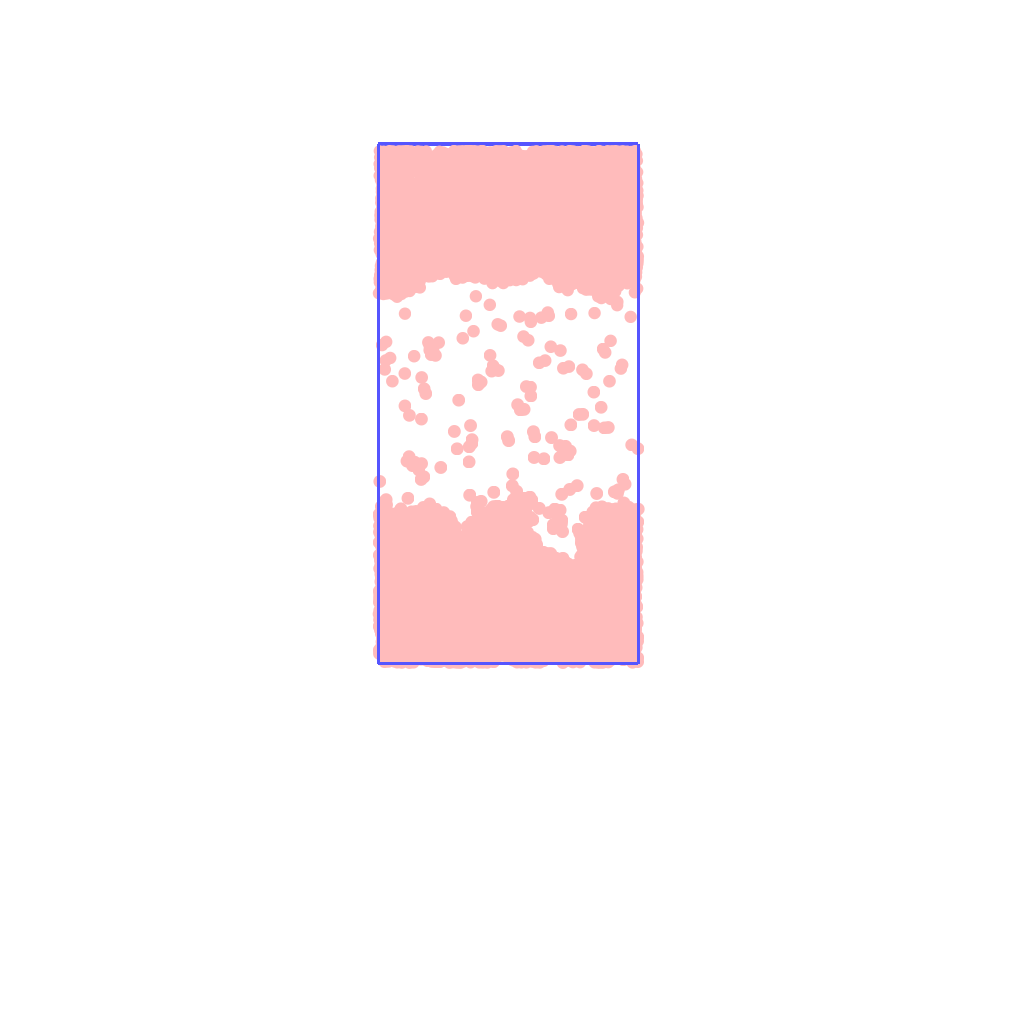
\includegraphics[scale=0.2]{image/2023-11-21T21:01:17.543_followup_chi1.265_Ay100_rho0.4_T0.43_dT0.04_Rd0.0_Rt0.5_Ra1.877538_g0.00019998593898298055_run1.0e8_output.png}}
  \caption{Ay100\_rho0.4\_T0.43\_dT0.04\_Rd0.0\_Rt0.5\_Ra1.877538\_g0.0004\_run1.0e8}
  \label{}
\end{figure}

\subsection{$\text{R}_\text{a}$, $\text{R}_\text{t}$ マップ}

$\text{R}_\text{a}$ と $\text{R}_\text{t}$ を少しずつ変えた系でシミュレーションをして, 粒子集団の様相の変化を見たい. 以下に示すのが, それらを動かす範囲である.

\begin{align}
  \text{R}_\text{a} &= 0.0 \sim 3.0 - 2^{1/6} = 1.877\dots \\
  \text{R}_\text{t} &= 0.0 \sim 0.5
\end{align}

\begin{figure}[H]
  \centering
  \begin{tabular}{ccccc}
    \begin{minipage}[t]{0.2\hsize}
      \centering
      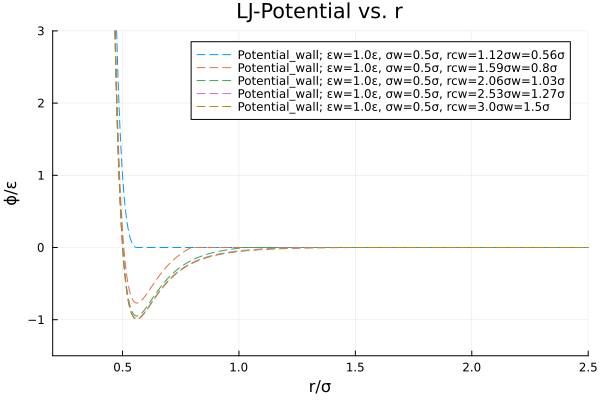
\includegraphics[width=\textwidth]{image/RaRtmap_LJ/LJ-Potential_Rt0.0.png}
      \subcaption{$\text{R}_\text{t}:0.0$}
      \label{}
    \end{minipage} &
    \begin{minipage}[t]{0.2\hsize}
      \centering
      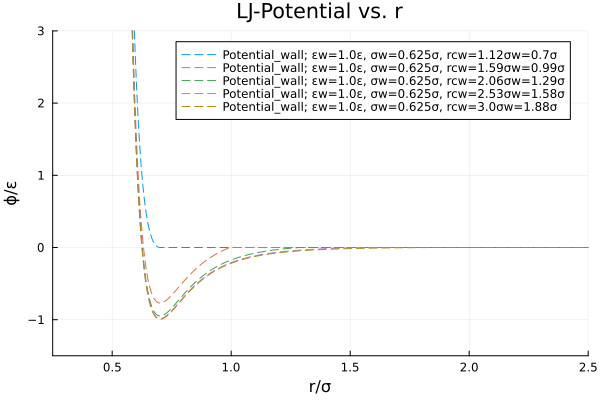
\includegraphics[width=\textwidth]{image/RaRtmap_LJ/LJ-Potential_Rt0.125.png}
      \subcaption{$\text{R}_\text{t}:0.125$}
      \label{}
    \end{minipage} &
    \begin{minipage}[t]{0.2\hsize}
      \centering
      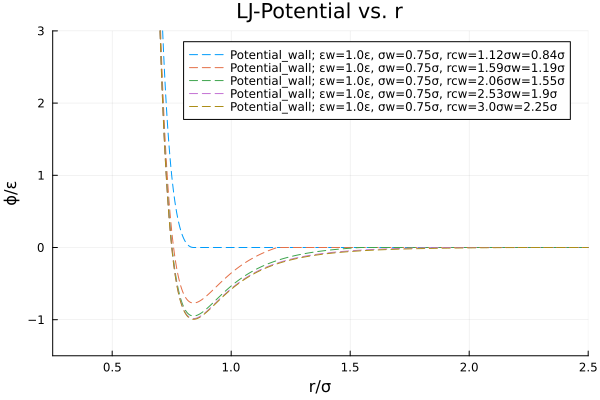
\includegraphics[width=\textwidth]{image/RaRtmap_LJ/LJ-Potential_Rt0.25.png}
      \subcaption{$\text{R}_\text{t}:0.25$}
      \label{}
    \end{minipage} &
    \begin{minipage}[t]{0.2\hsize}
      \centering
      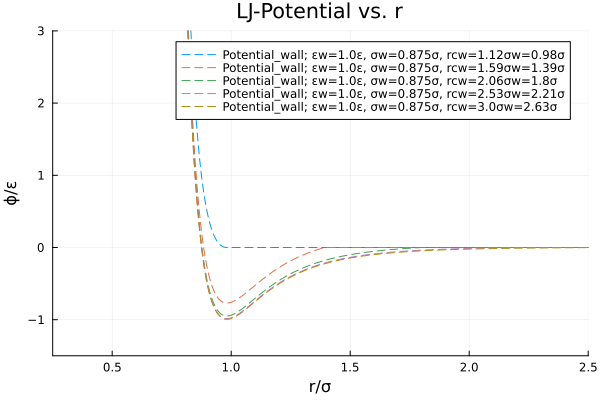
\includegraphics[width=\textwidth]{image/RaRtmap_LJ/LJ-Potential_Rt0.375.png}
      \subcaption{$\text{R}_\text{t}:0.375$}
      \label{}
    \end{minipage} &
    \begin{minipage}[t]{0.2\hsize}
      \centering
      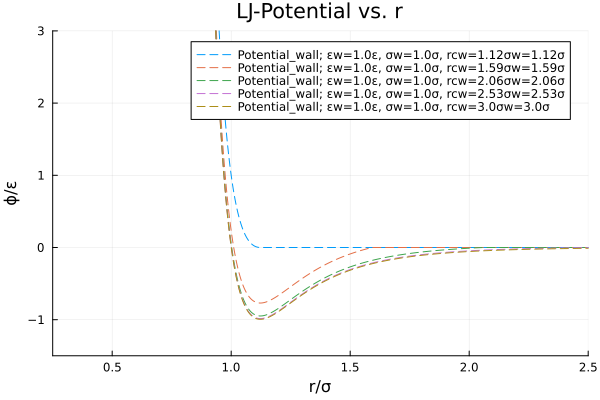
\includegraphics[width=\textwidth]{image/RaRtmap_LJ/LJ-Potential_Rt0.5.png}
      \subcaption{$\text{R}_\text{t}:0.5$}
      \label{}
    \end{minipage} 
  \end{tabular}
  \caption{LJ-potential}
  \label{}
\end{figure}

パラメータを確認.

\begin{itemize}
  \item $N = 1250$
  \item $\rho {\sigma}^2 = 0.4$
  \item $L_x / \sigma = 39.5\dots$
  \item $L_y / \sigma = 79.0\dots$
  \item $k_{\text{B}} T / \varepsilon = 0.43$
  \item $k_{\text{B}} \Delta T / \varepsilon = 0.04$
  \item $mg\sigma/\varepsilon = 4.0 \times 10^{-4}$
  \item $t_f \sqrt{\varepsilon / m \sigma^2} = 2.0 \times 10^{5}$
\end{itemize}

\begin{figure}[H]
  \begin{tabular}{ccccc}
    \begin{minipage}[t]{0.2\hsize}
      \centering
      \href{https://youtu.be/yc-GeIQBuCk}{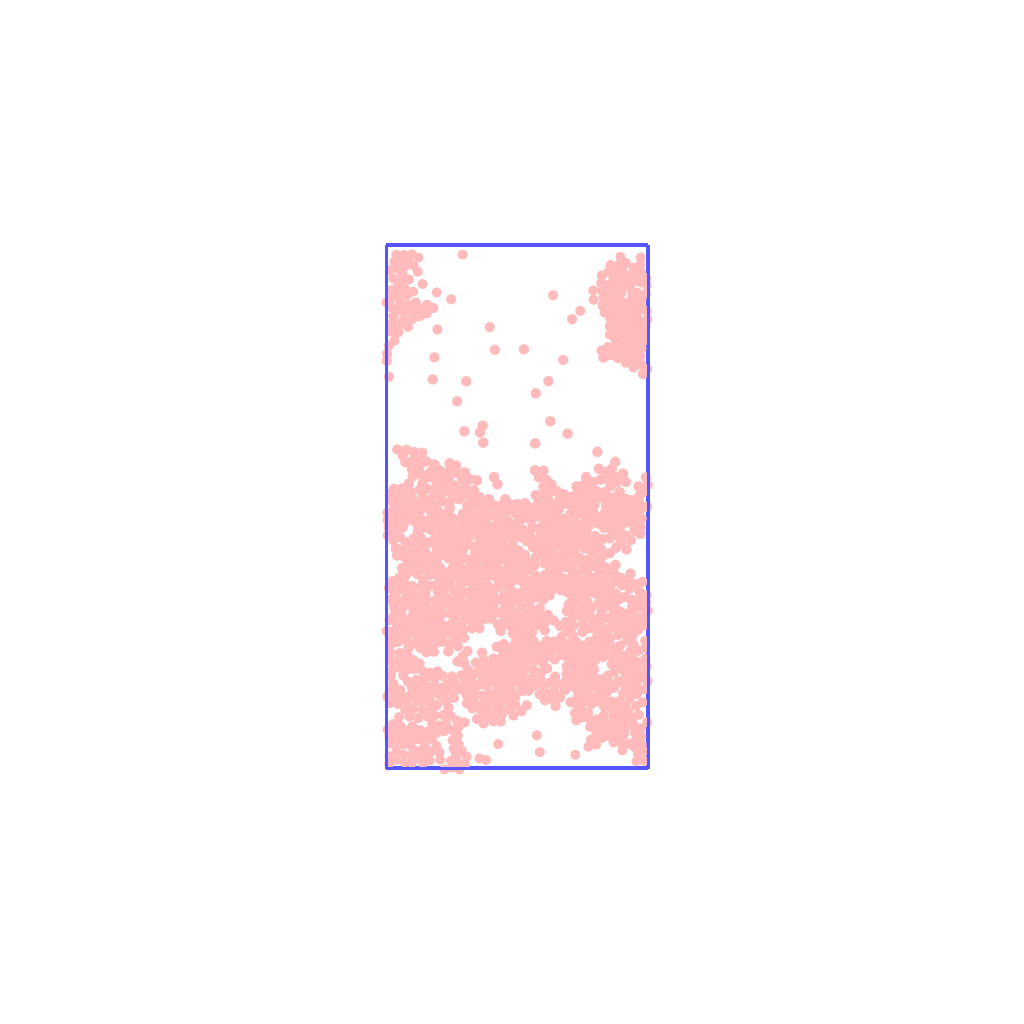
\includegraphics[width=\textwidth]{image/RaRtmap/2023-11-14T18:19:29.358__chi1.265_Ay50_rho0.4_T0.43_dT0.04_Rd0.0_Rt0.0_Ra0.0_g0.0003999718779659611_run4.0e7_output.png}}
      \subcaption{$\text{R}_\text{a}=0.0,\\\text{R}_\text{t}=0.0$}
      % \label{}
    \end{minipage} &
    \begin{minipage}[t]{0.2\hsize}
      \centering
      \href{https://youtu.be/4rNNLx9_DZ4}{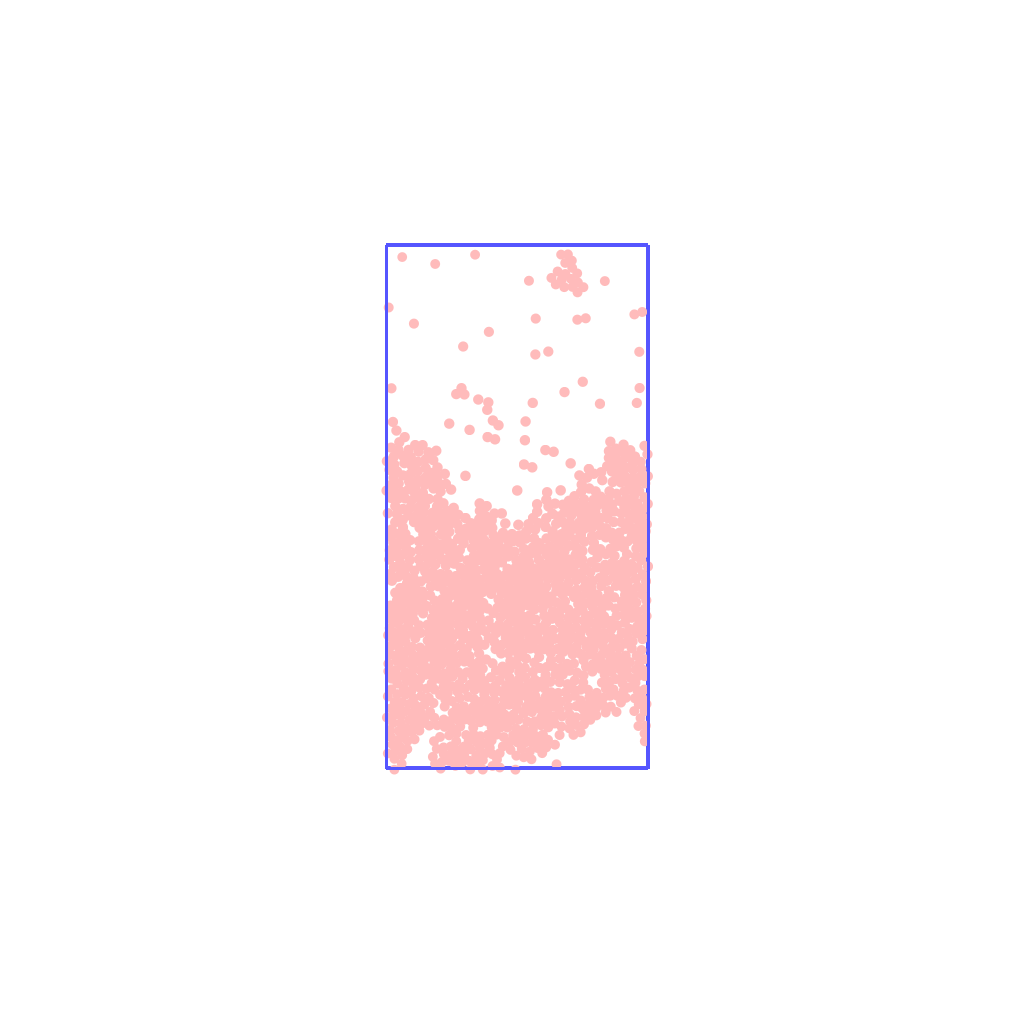
\includegraphics[width=\textwidth]{image/RaRtmap/2023-11-14T19:14:52.710__chi1.265_Ay50_rho0.4_T0.43_dT0.04_Rd0.0_Rt0.0_Ra0.4693845_g0.0003999718779659611_run4.0e7_output.png}}
      \subcaption{$\text{R}_\text{a}=0.469,\\\text{R}_\text{t}=0.0$}
      % \label{}
    \end{minipage} &
    \begin{minipage}[t]{0.2\hsize}
      \centering
      \href{https://youtu.be/QKLz7NzBte8}{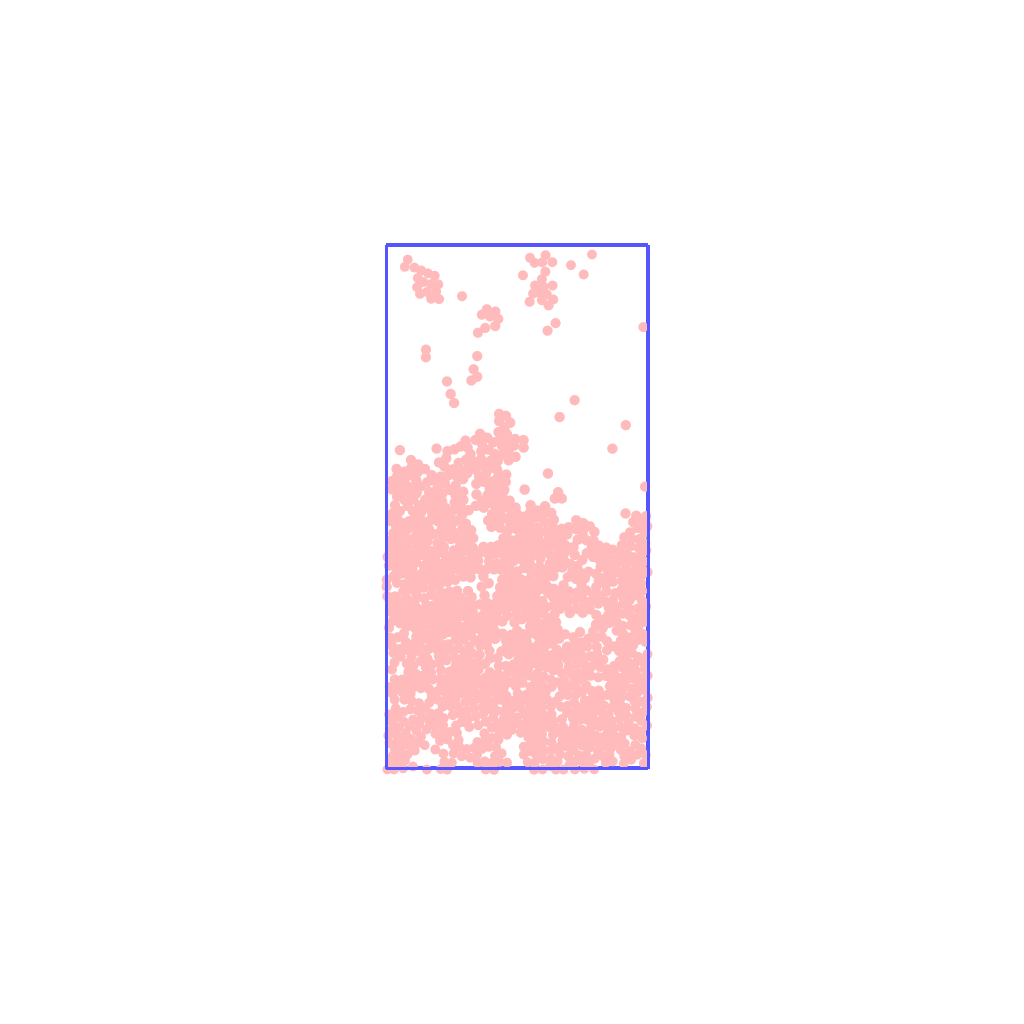
\includegraphics[width=\textwidth]{image/RaRtmap/2023-11-14T20:07:58.625__chi1.265_Ay50_rho0.4_T0.43_dT0.04_Rd0.0_Rt0.0_Ra0.938769_g0.0003999718779659611_run4.0e7_output.png}}
      \subcaption{$\text{R}_\text{a}=0.938,\\\text{R}_\text{t}=0.0$}
      % \label{}
    \end{minipage} &
    \begin{minipage}[t]{0.2\hsize}
      \centering
      \href{https://youtu.be/6iqcv_Af2U8}{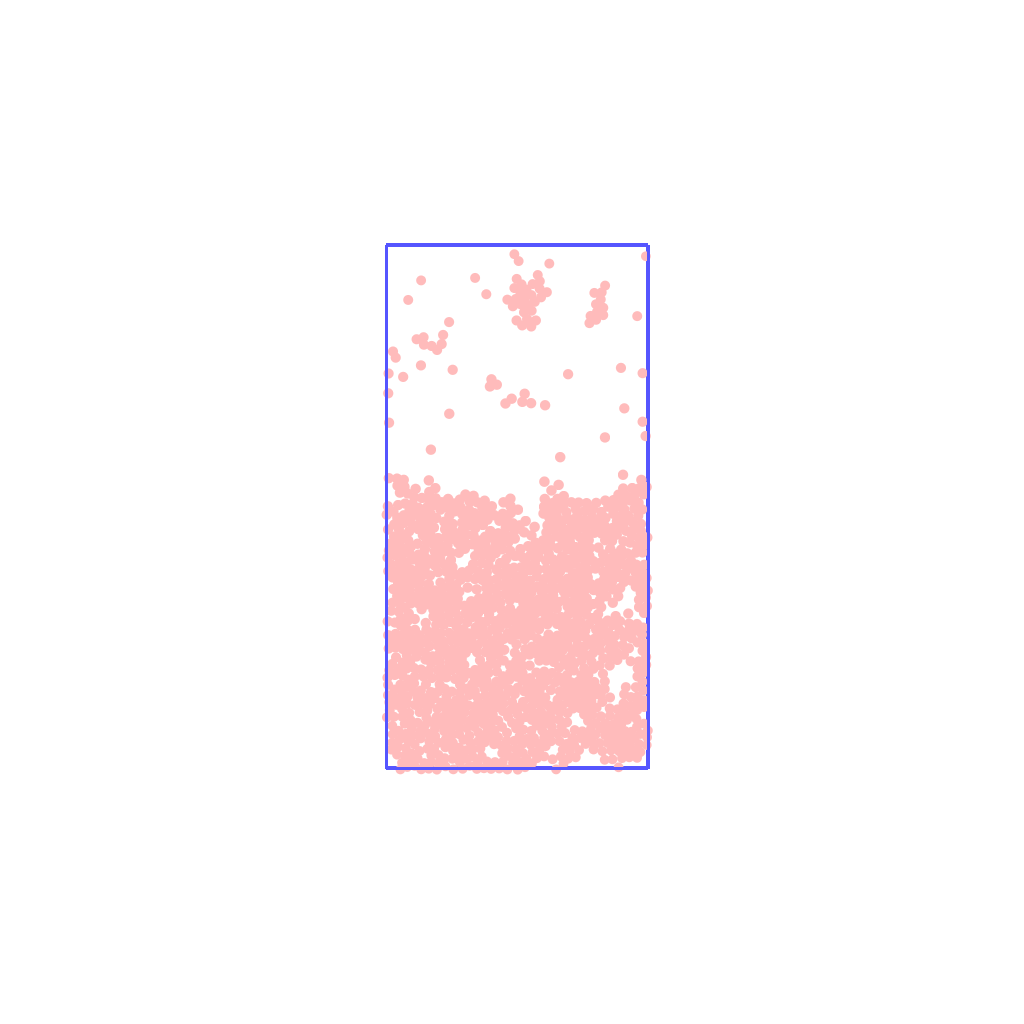
\includegraphics[width=\textwidth]{image/RaRtmap/2023-11-14T21:01:09.992__chi1.265_Ay50_rho0.4_T0.43_dT0.04_Rd0.0_Rt0.0_Ra1.4081535_g0.0003999718779659611_run4.0e7_output.png}}
      \subcaption{$\text{R}_\text{a}=1.408,\\\text{R}_\text{t}=0.0$}
      % \label{}
    \end{minipage} &
    \begin{minipage}[t]{0.2\hsize}
      \centering
      \href{https://youtu.be/Tn1Hd2eR0yo}{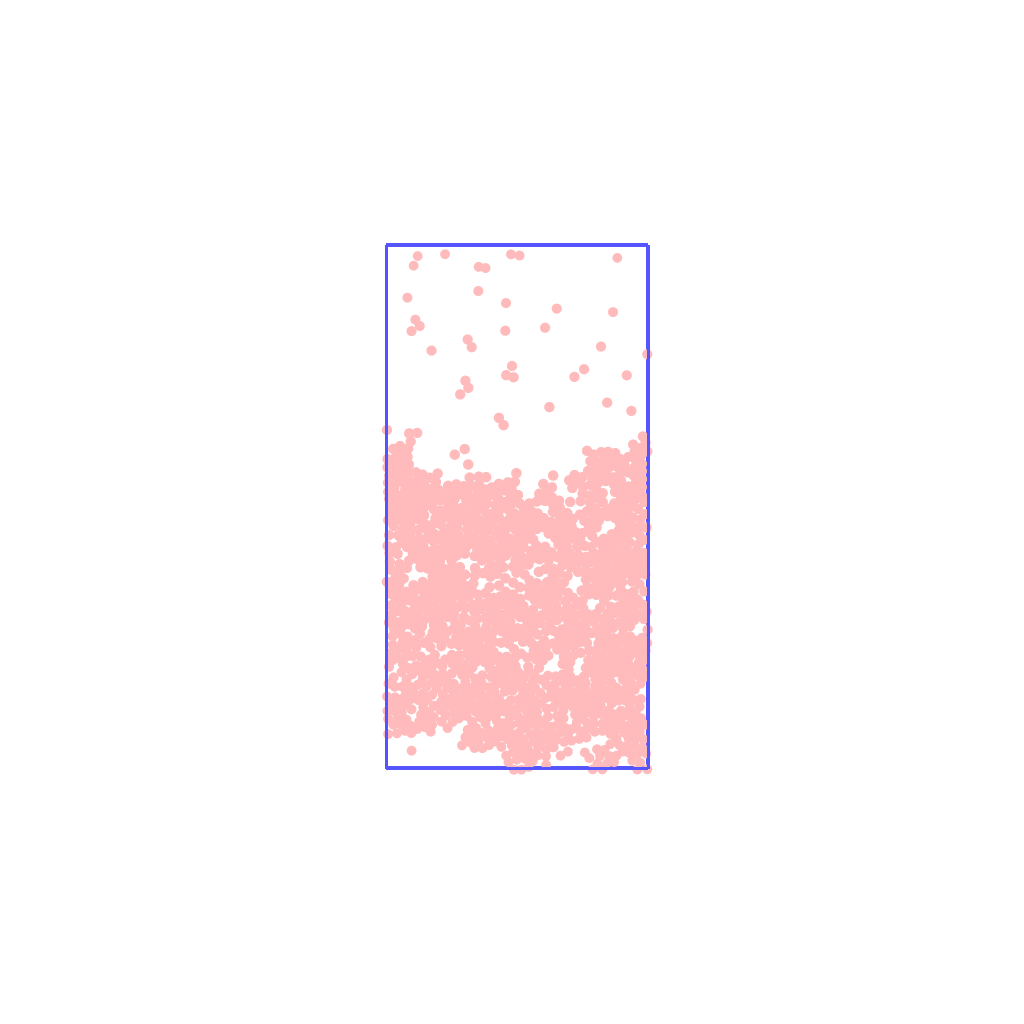
\includegraphics[width=\textwidth]{image/RaRtmap/2023-11-14T21:54:59.835__chi1.265_Ay50_rho0.4_T0.43_dT0.04_Rd0.0_Rt0.0_Ra1.877538_g0.0003999718779659611_run4.0e7_output.png}}
      \subcaption{$\text{R}_\text{a}=1.877,\\\text{R}_\text{t}=0.0$}
      % \label{}
    \end{minipage} \\
    \begin{minipage}[t]{0.2\hsize}
      \centering
      \href{https://youtu.be/B1GwQFCBszs}{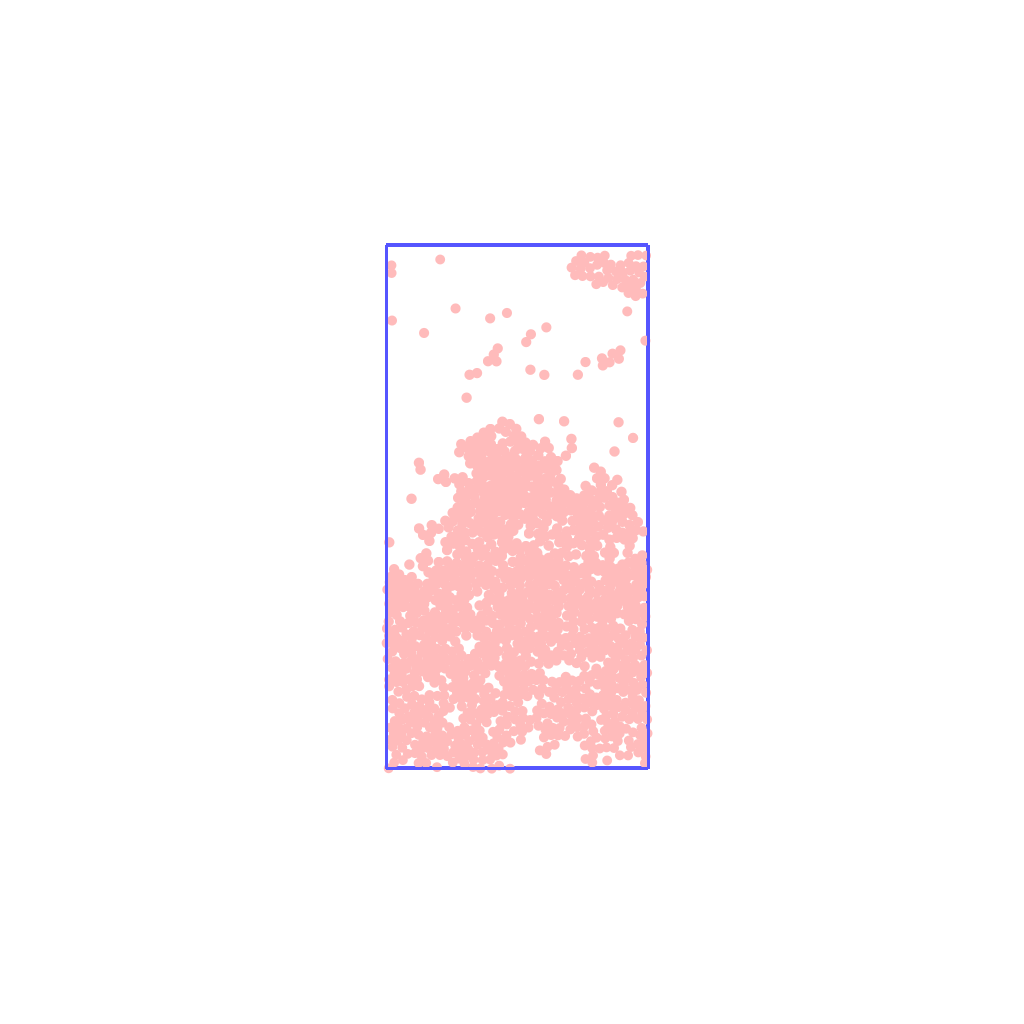
\includegraphics[width=\textwidth]{image/RaRtmap/2023-11-14T22:51:24.191__chi1.265_Ay50_rho0.4_T0.43_dT0.04_Rd0.0_Rt0.125_Ra0.0_g0.0003999718779659611_run4.0e7_output.png}}
      \subcaption{$\text{R}_\text{a}=0.0,\\\text{R}_\text{t}=0.125$}
      % \label{}
    \end{minipage} &
    \begin{minipage}[t]{0.2\hsize}
      \centering
      \href{https://youtu.be/MRIfAketXOI}{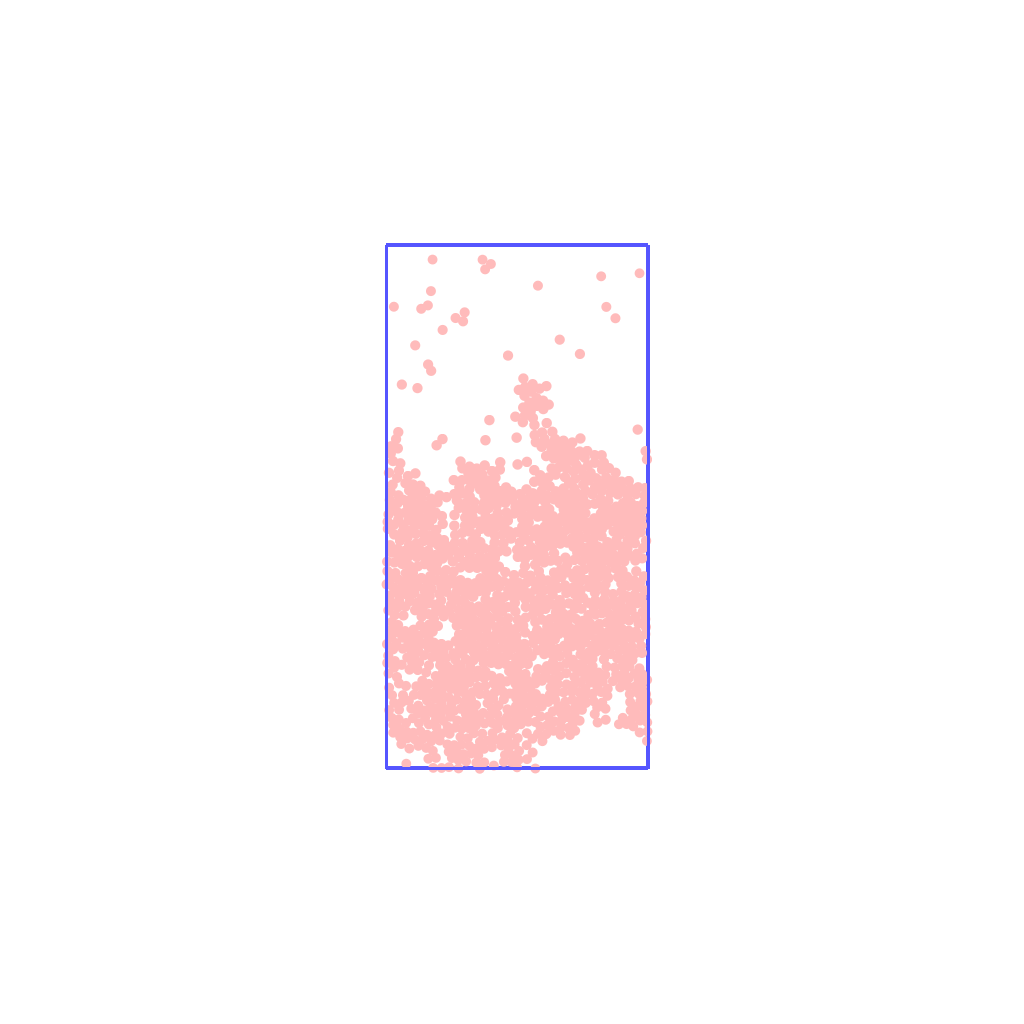
\includegraphics[width=\textwidth]{image/RaRtmap/2023-11-14T23:48:31.439__chi1.265_Ay50_rho0.4_T0.43_dT0.04_Rd0.0_Rt0.125_Ra0.4693845_g0.0003999718779659611_run4.0e7_output.png}}
      \subcaption{$\text{R}_\text{a}=0.469,\\\text{R}_\text{t}=0.125$}
      % \label{}
    \end{minipage} &
    \begin{minipage}[t]{0.2\hsize}
      \centering
      \href{https://youtu.be/v7rYxdoSSjI}{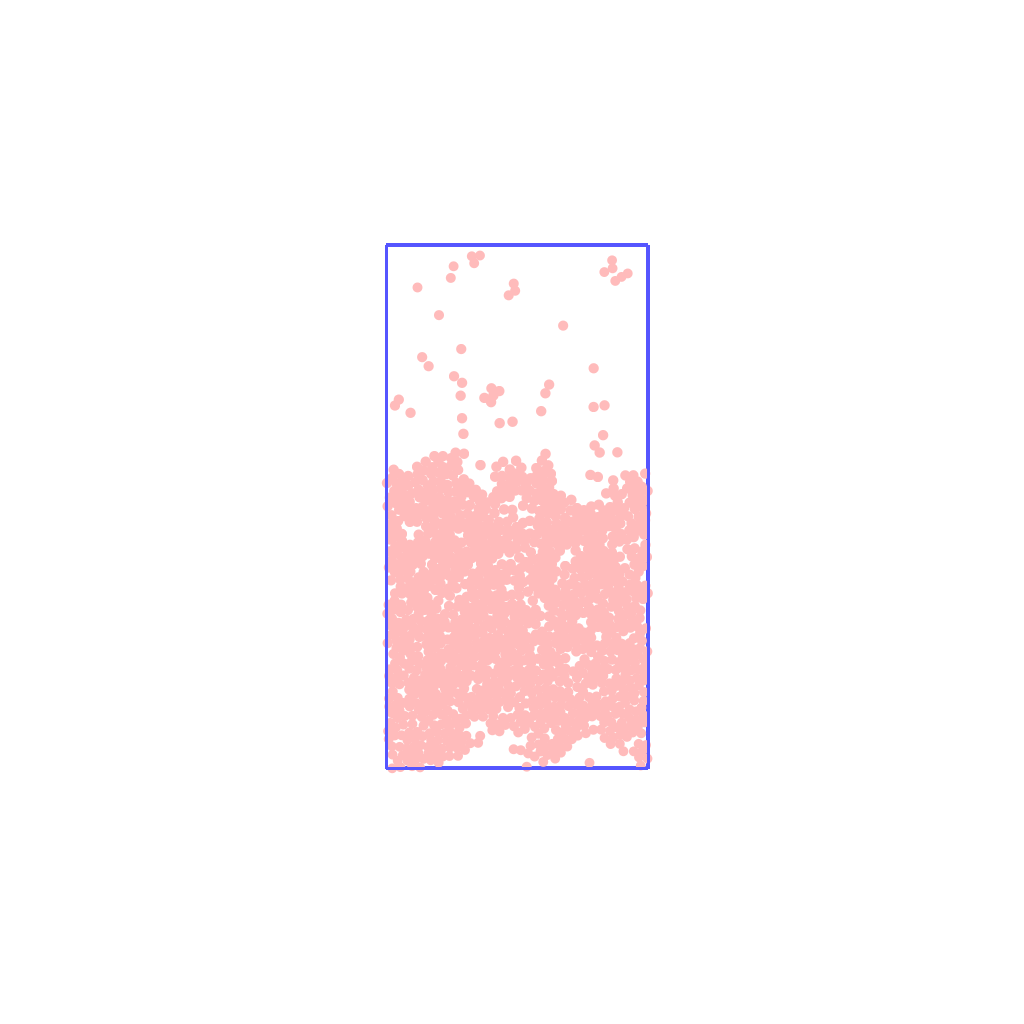
\includegraphics[width=\textwidth]{image/RaRtmap/2023-11-15T00:43:33.781__chi1.265_Ay50_rho0.4_T0.43_dT0.04_Rd0.0_Rt0.125_Ra0.938769_g0.0003999718779659611_run4.0e7_output.png}}
      \subcaption{$\text{R}_\text{a}=0.938,\\\text{R}_\text{t}=0.125$}
      % \label{}
    \end{minipage} &
    \begin{minipage}[t]{0.2\hsize}
      \centering
      \href{https://youtu.be/0NFYPFYBcc4}{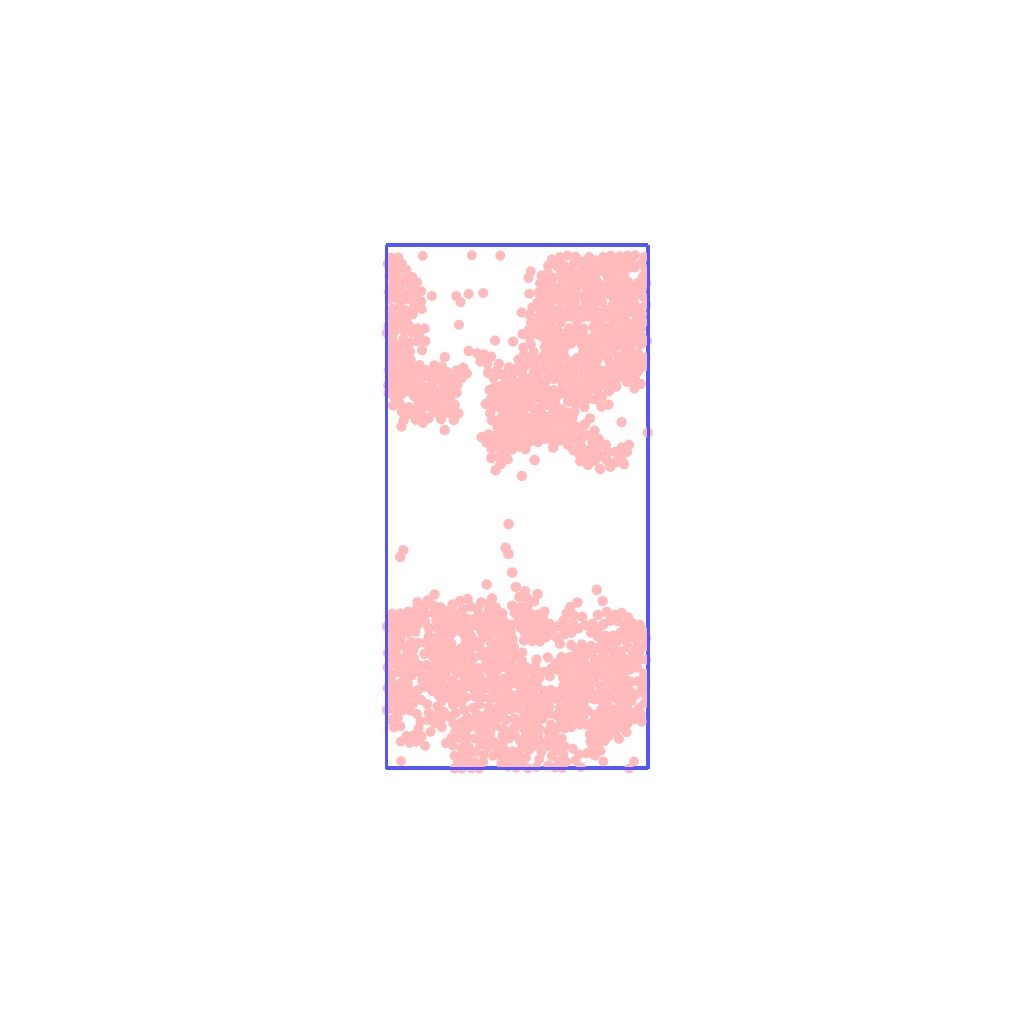
\includegraphics[width=\textwidth]{image/RaRtmap/2023-11-15T01:35:17.404__chi1.265_Ay50_rho0.4_T0.43_dT0.04_Rd0.0_Rt0.125_Ra1.4081535_g0.0003999718779659611_run4.0e7_output.png}}
      \subcaption{$\text{R}_\text{a}=1.408,\\\text{R}_\text{t}=0.125$}
      % \label{}
    \end{minipage} &
    \begin{minipage}[t]{0.2\hsize}
      \centering
      \href{https://youtu.be/FXTDOcpARl0}{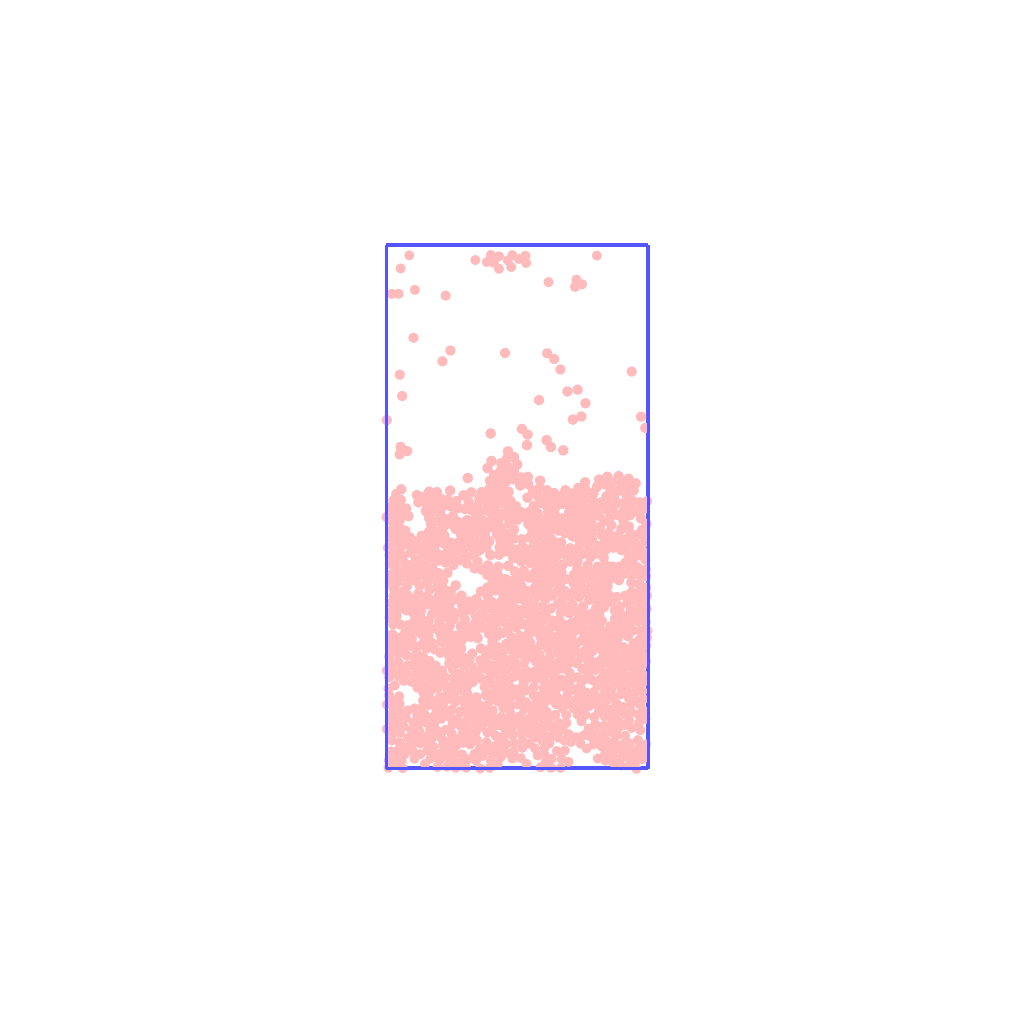
\includegraphics[width=\textwidth]{image/RaRtmap/2023-11-15T02:27:34.337__chi1.265_Ay50_rho0.4_T0.43_dT0.04_Rd0.0_Rt0.125_Ra1.877538_g0.0003999718779659611_run4.0e7_output.png}}
      \subcaption{$\text{R}_\text{a}=1.877,\\\text{R}_\text{t}=0.125$}
      % \label{}
    \end{minipage} \\
    \begin{minipage}[t]{0.2\hsize}
      \centering
      \href{https://youtu.be/4A\_MHNHZrKQ}{
      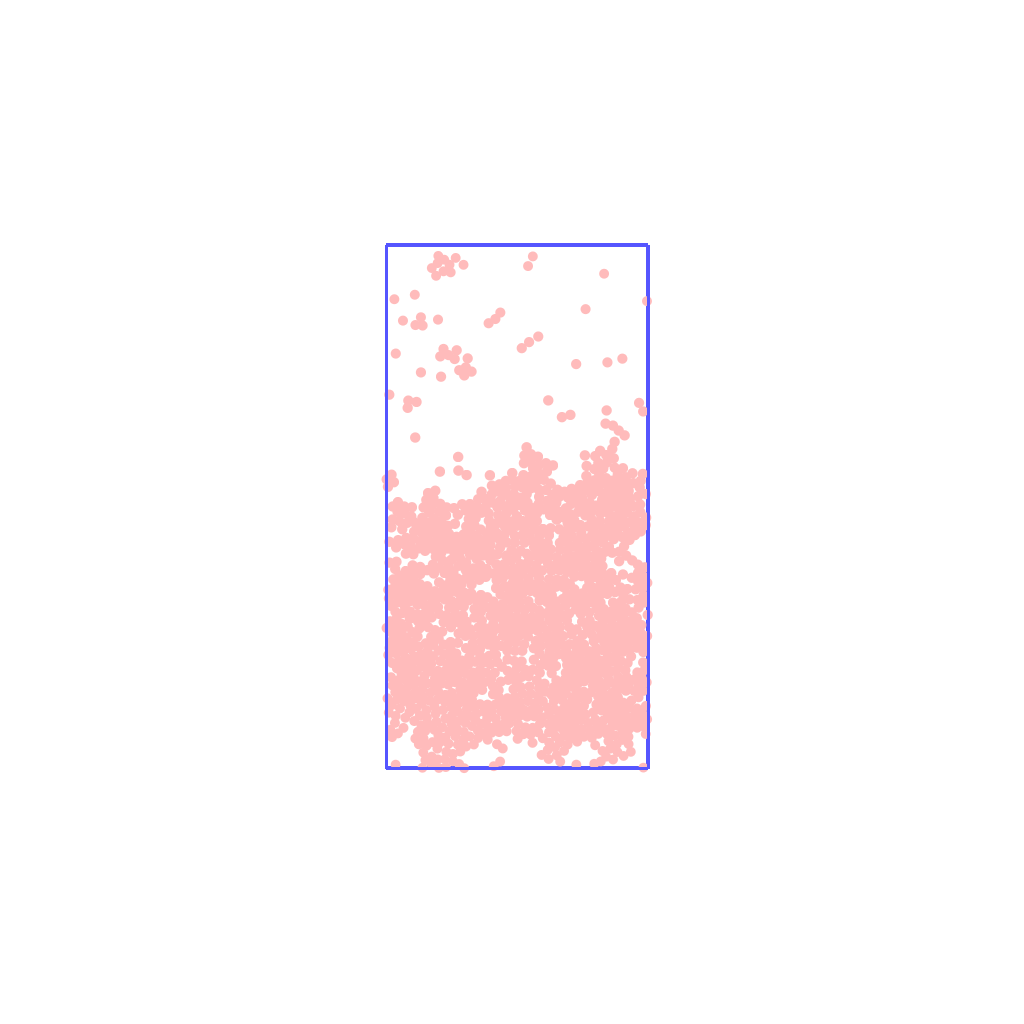
\includegraphics[width=\textwidth]{image/RaRtmap/2023-11-15T03:19:32.715__chi1.265_Ay50_rho0.4_T0.43_dT0.04_Rd0.0_Rt0.25_Ra0.0_g0.0003999718779659611_run4.0e7_output.png}}
      \subcaption{$\text{R}_\text{a}=0.0,\\\text{R}_\text{t}=0.250$}
      % \label{}
    \end{minipage} &
    \begin{minipage}[t]{0.2\hsize}
      \centering
      \href{https://youtu.be/jGzUPm\_3oH0}{
      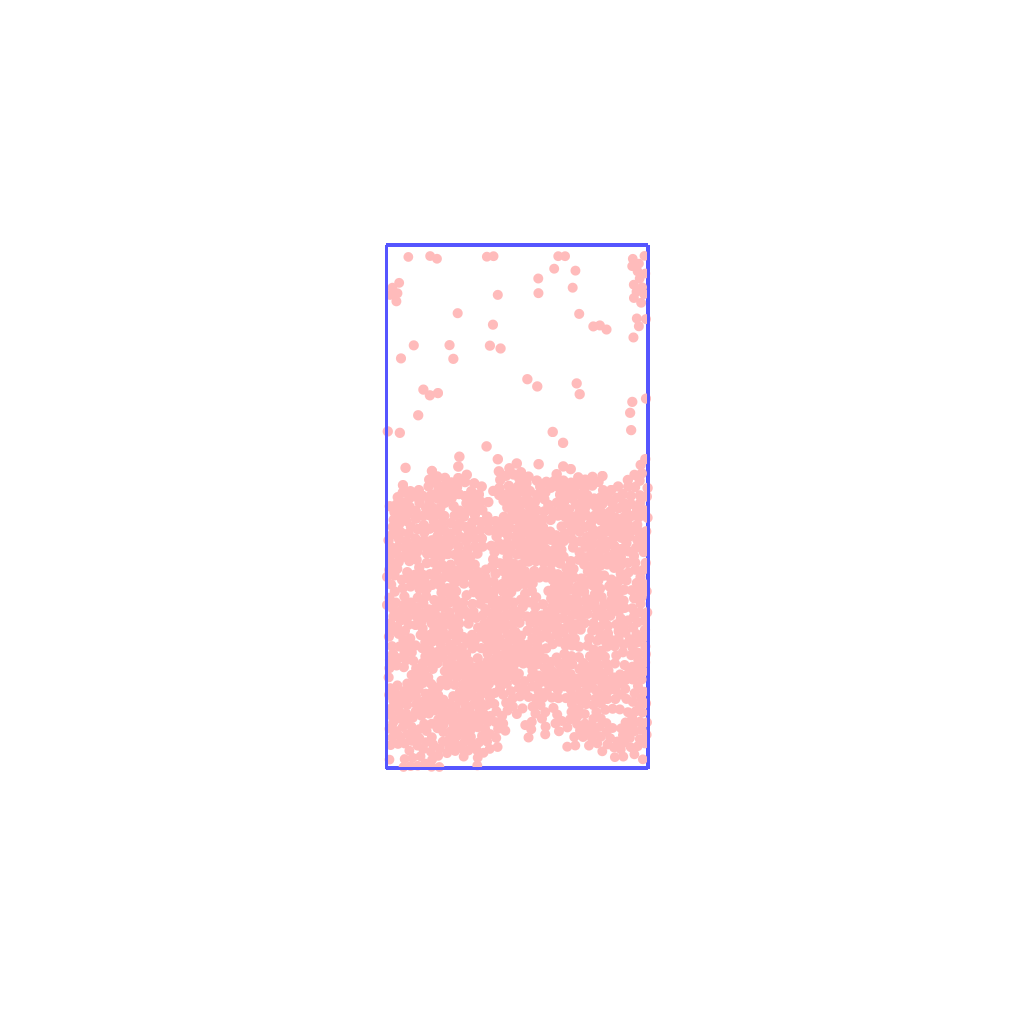
\includegraphics[width=\textwidth]{image/RaRtmap/2023-11-15T04:11:00.956__chi1.265_Ay50_rho0.4_T0.43_dT0.04_Rd0.0_Rt0.25_Ra0.4693845_g0.0003999718779659611_run4.0e7_output.png}}
      \subcaption{$\text{R}_\text{a}=0.469,\\\text{R}_\text{t}=0.250$}
      % \label{}
    \end{minipage} &
    \begin{minipage}[t]{0.2\hsize}
      \centering
      \href{https://youtu.be/0iyDEBwDF7A}{
      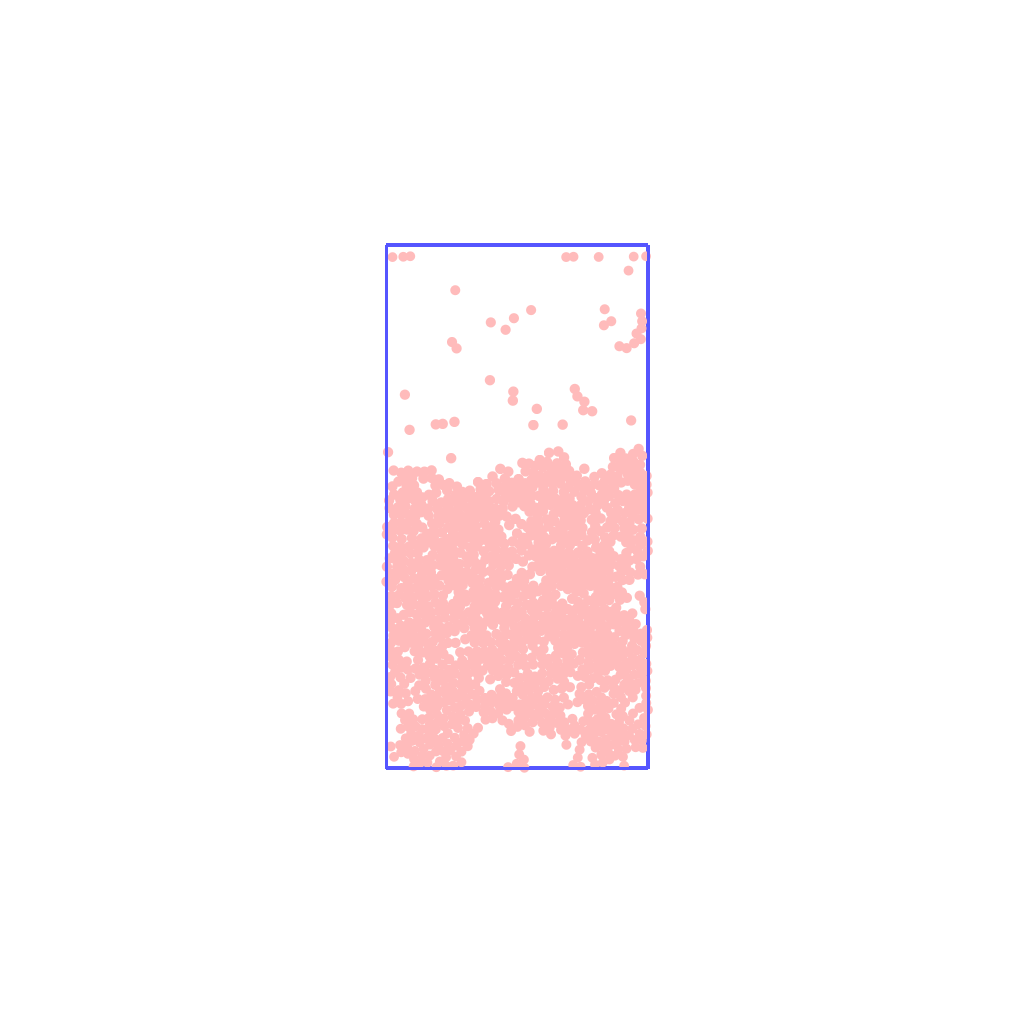
\includegraphics[width=\textwidth]{image/RaRtmap/2023-11-15T05:03:45.973__chi1.265_Ay50_rho0.4_T0.43_dT0.04_Rd0.0_Rt0.25_Ra0.938769_g0.0003999718779659611_run4.0e7_output.png}}
      \subcaption{$\text{R}_\text{a}=0.938,\\\text{R}_\text{t}=0.250$}
      % \label{}
    \end{minipage} &
    \begin{minipage}[t]{0.2\hsize}
      \centering
      \href{https://youtu.be/Sqk3HDSDINw}{
      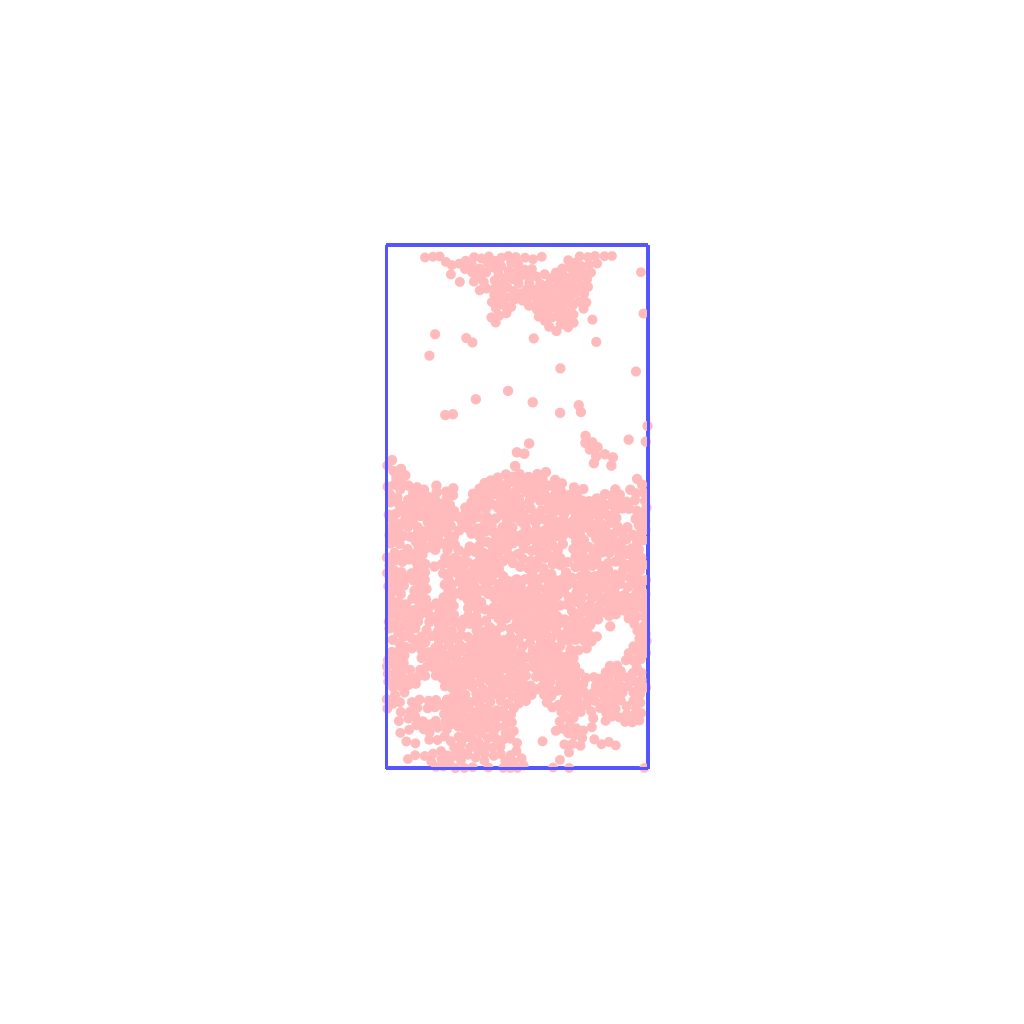
\includegraphics[width=\textwidth]{image/RaRtmap/2023-11-15T05:53:00.667__chi1.265_Ay50_rho0.4_T0.43_dT0.04_Rd0.0_Rt0.25_Ra1.4081535_g0.0003999718779659611_run4.0e7_output.png}}
      \subcaption{$\text{R}_\text{a}=1.408,\\\text{R}_\text{t}=0.250$}
      % \label{}
    \end{minipage} &
    \begin{minipage}[t]{0.2\hsize}
      \centering
      \href{https://youtu.be/3lqCLQchVYA}{
      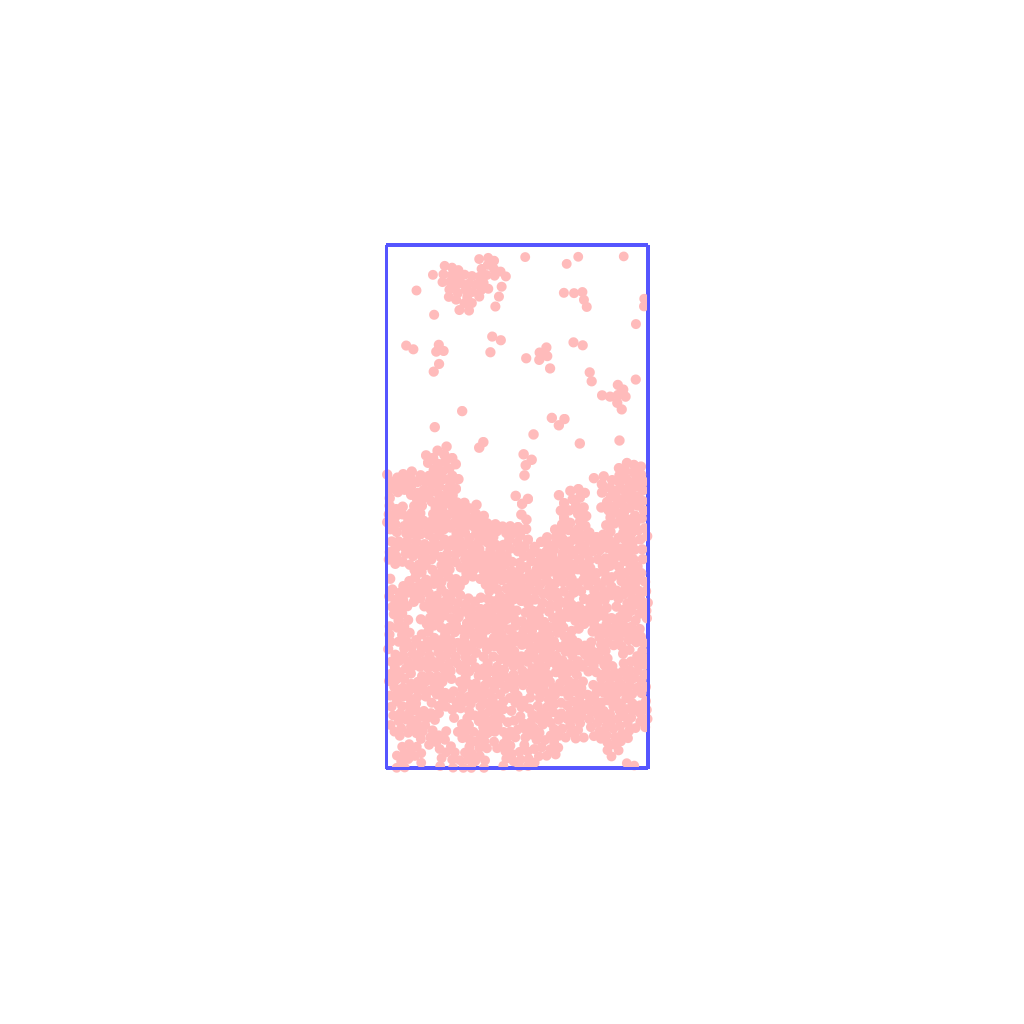
\includegraphics[width=\textwidth]{image/RaRtmap/2023-11-15T06:43:21.554__chi1.265_Ay50_rho0.4_T0.43_dT0.04_Rd0.0_Rt0.25_Ra1.877538_g0.0003999718779659611_run4.0e7_output.png}}
      \subcaption{$\text{R}_\text{a}=1.877,\\\text{R}_\text{t}=0.250$}
      % \label{}
    \end{minipage} \\
    \begin{minipage}[t]{0.2\hsize}
      \centering
      \href{https://youtu.be/1cMmZVmcThA}{
      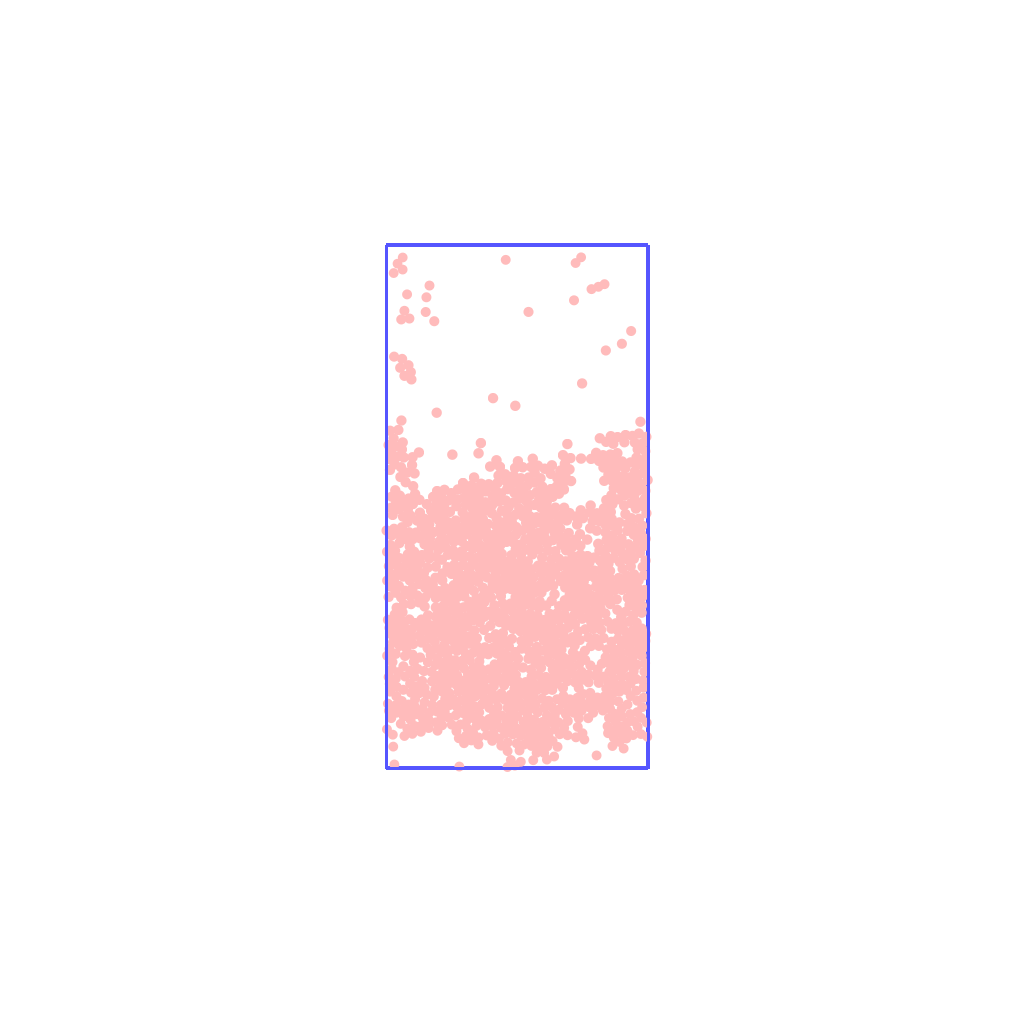
\includegraphics[width=\textwidth]{image/RaRtmap/2023-11-15T07:34:00.555__chi1.265_Ay50_rho0.4_T0.43_dT0.04_Rd0.0_Rt0.375_Ra0.0_g0.0003999718779659611_run4.0e7_output.png}}
      \subcaption{$\text{R}_\text{a}=0.0,\\\text{R}_\text{t}=0.375$}
      % \label{}
    \end{minipage} &
    \begin{minipage}[t]{0.2\hsize}
      \centering
      \href{https://youtu.be/MDWWS7Axo-4}{
      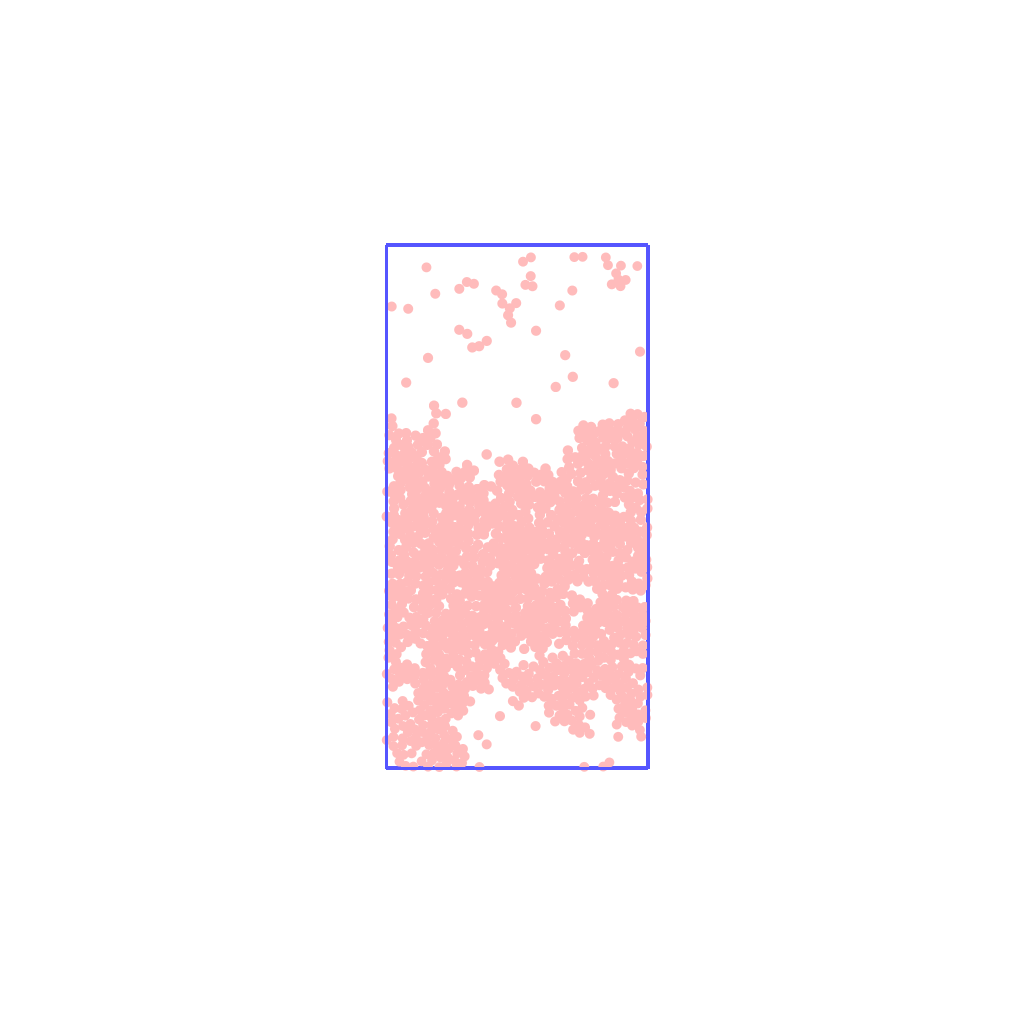
\includegraphics[width=\textwidth]{image/RaRtmap/2023-11-15T08:24:37.362__chi1.265_Ay50_rho0.4_T0.43_dT0.04_Rd0.0_Rt0.375_Ra0.4693845_g0.0003999718779659611_run4.0e7_output.png}}
      \subcaption{$\text{R}_\text{a}=0.469,\\\text{R}_\text{t}=0.375$}
      % \label{}
    \end{minipage} &
    \begin{minipage}[t]{0.2\hsize}
      \centering
      \href{https://youtu.be/Y6O_tVs6mHY}{
      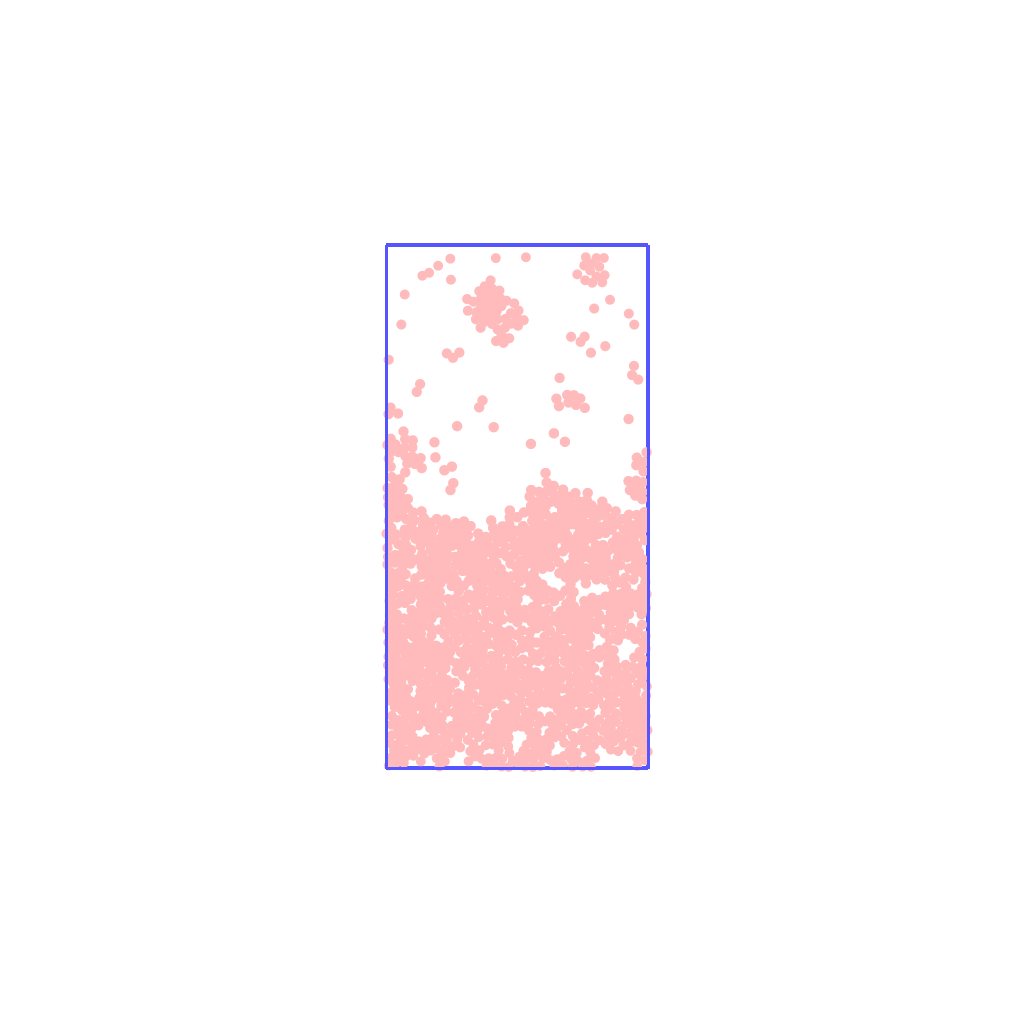
\includegraphics[width=\textwidth]{image/RaRtmap/2023-11-15T09:16:40.082__chi1.265_Ay50_rho0.4_T0.43_dT0.04_Rd0.0_Rt0.375_Ra0.938769_g0.0003999718779659611_run4.0e7_output.png}}
      \subcaption{$\text{R}_\text{a}=0.938,\\\text{R}_\text{t}=0.375$}
      % \label{}
    \end{minipage} &
    \begin{minipage}[t]{0.2\hsize}
      \centering
      \href{https://youtu.be/yeI5CDT0TEw}{
      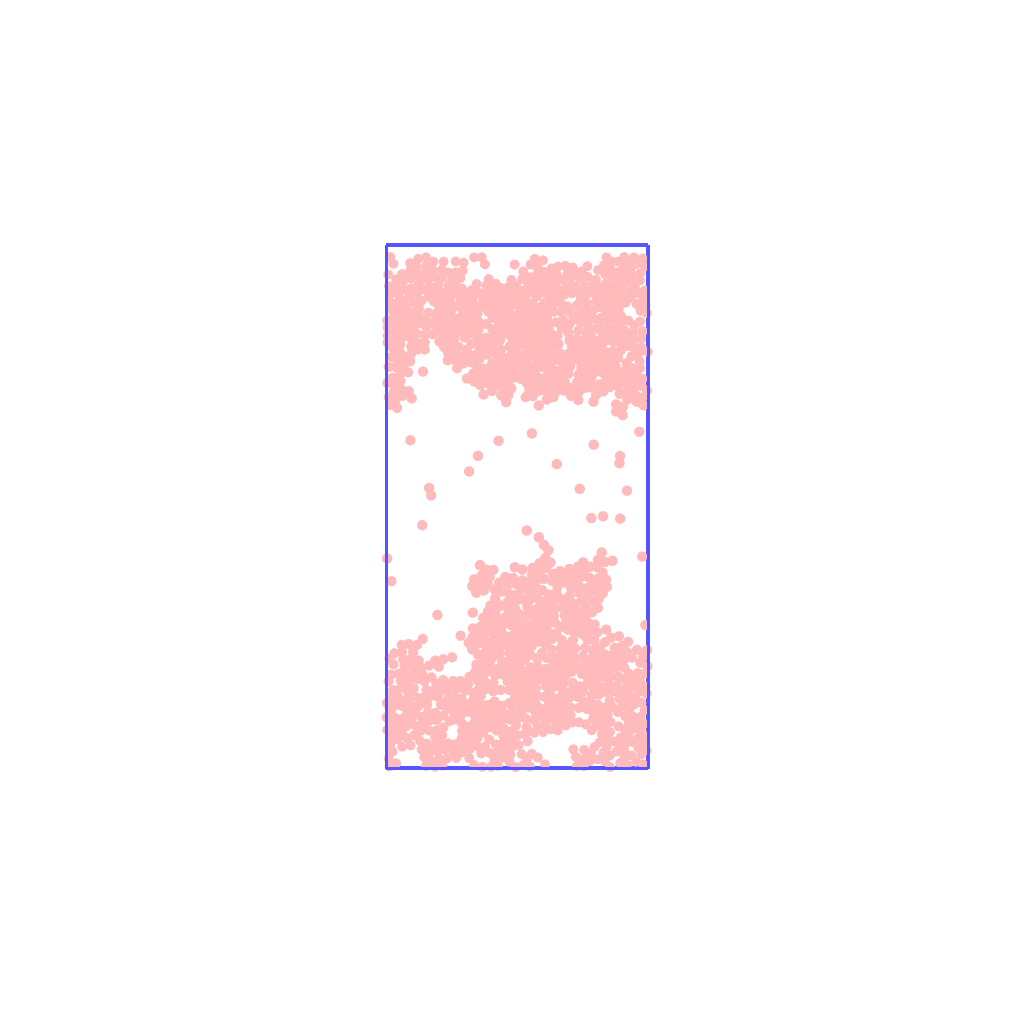
\includegraphics[width=\textwidth]{image/RaRtmap/2023-11-15T10:07:20.945__chi1.265_Ay50_rho0.4_T0.43_dT0.04_Rd0.0_Rt0.375_Ra1.4081535_g0.0003999718779659611_run4.0e7_output.png}}
      \subcaption{$\text{R}_\text{a}=1.408,\\\text{R}_\text{t}=0.375$}
      % \label{}
    \end{minipage} &
    \begin{minipage}[t]{0.2\hsize}
      \centering
      \href{https://youtu.be/h6w-DYqP-bg}{
      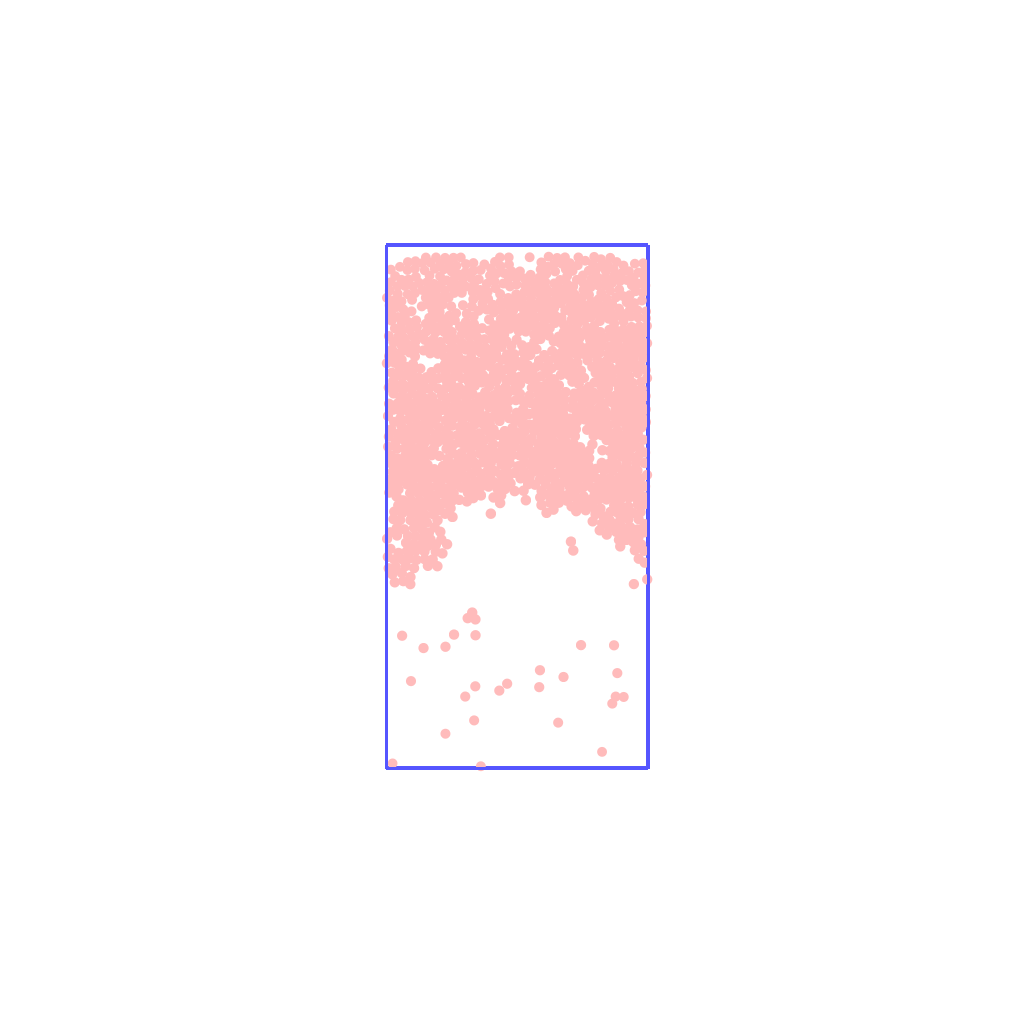
\includegraphics[width=\textwidth]{image/RaRtmap/2023-11-15T10:59:30.665__chi1.265_Ay50_rho0.4_T0.43_dT0.04_Rd0.0_Rt0.375_Ra1.877538_g0.0003999718779659611_run4.0e7_output.png}}
      \subcaption{$\text{R}_\text{a}=1.877,\\\text{R}_\text{t}=0.375$}
      % \label{}
    \end{minipage} \\
    \begin{minipage}[t]{0.2\hsize}
      \centering
      \href{https://youtu.be/S0NOYiYNCBU}{
      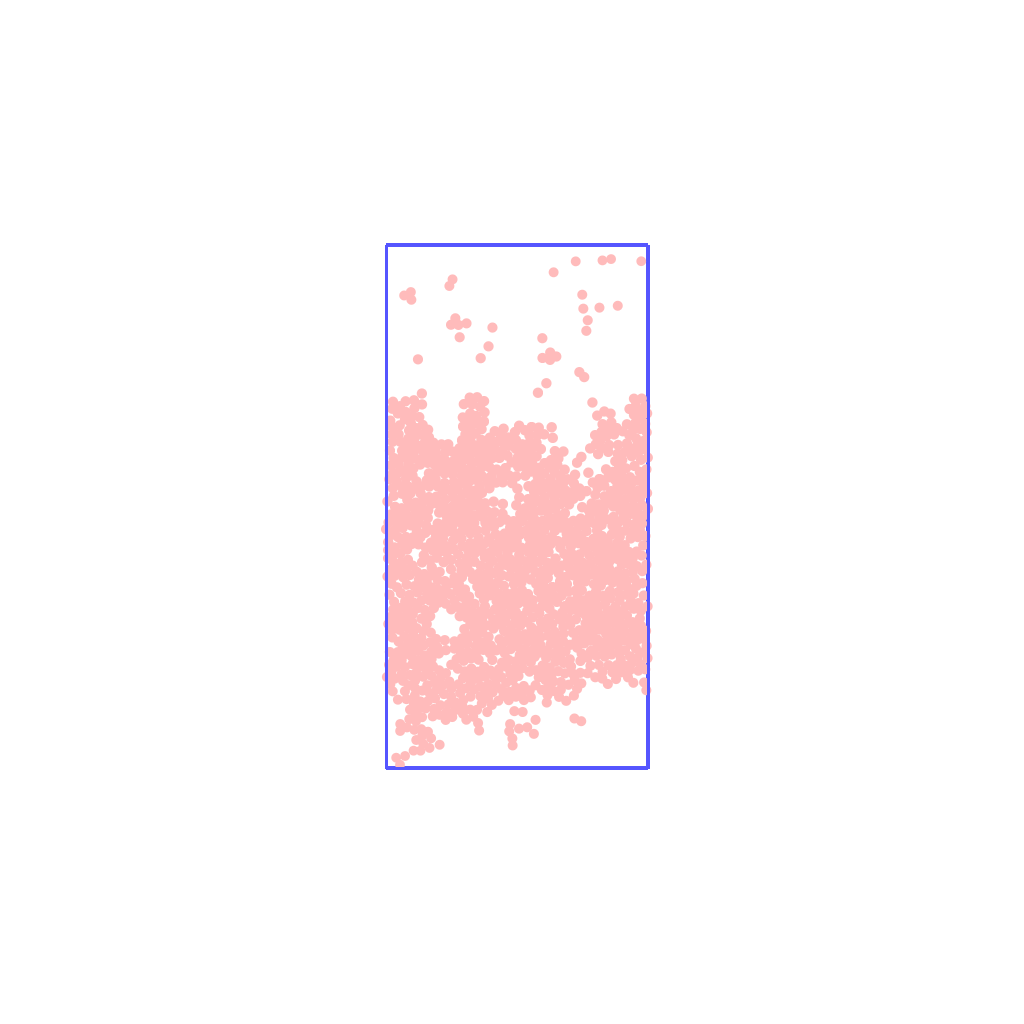
\includegraphics[width=\textwidth]{image/RaRtmap/2023-11-15T11:53:37.697__chi1.265_Ay50_rho0.4_T0.43_dT0.04_Rd0.0_Rt0.5_Ra0.0_g0.0003999718779659611_run4.0e7_output.png}}
      \subcaption{$\text{R}_\text{a}=0.0,\\\text{R}_\text{t}=0.500$}
      % \label{}
    \end{minipage} &
    \begin{minipage}[t]{0.2\hsize}
      \centering
      \href{https://youtu.be/l8Mz0kOFZwY}{
      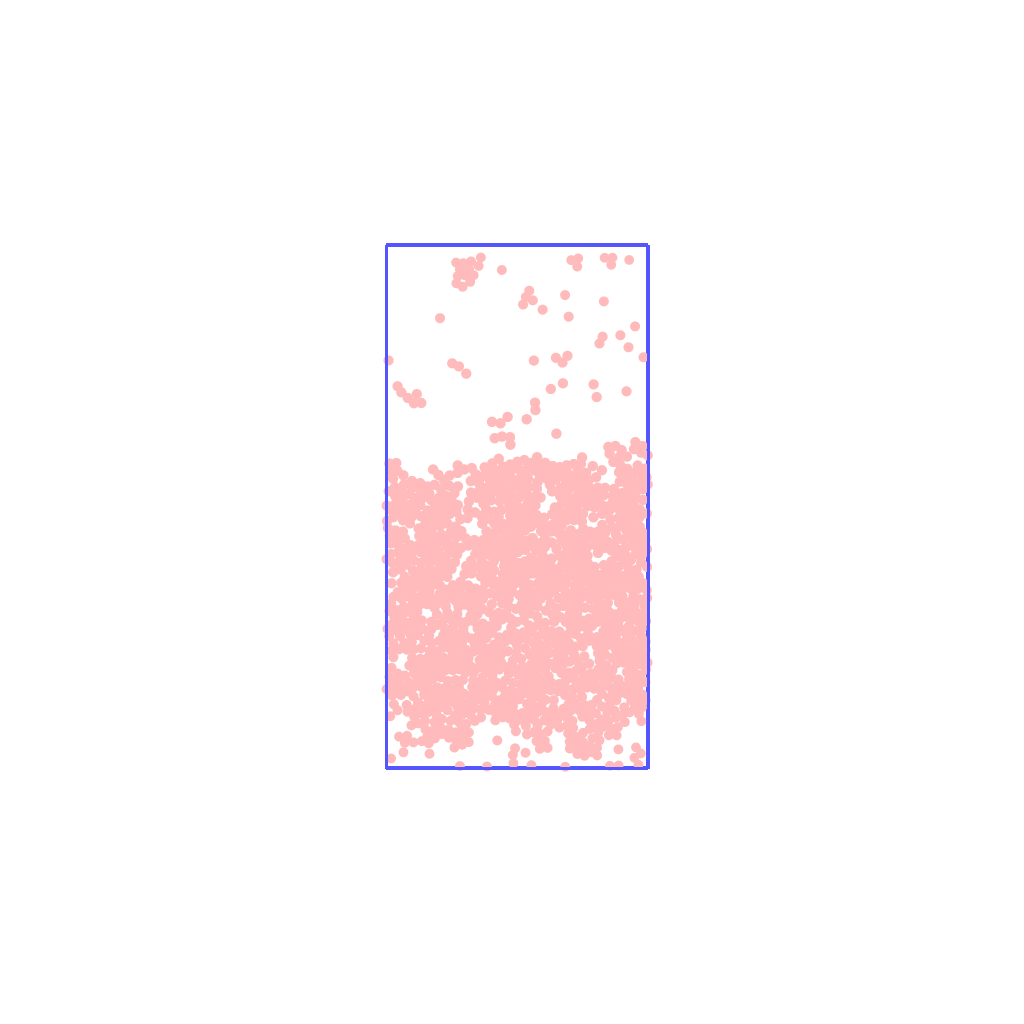
\includegraphics[width=\textwidth]{image/RaRtmap/2023-11-15T12:45:26.303__chi1.265_Ay50_rho0.4_T0.43_dT0.04_Rd0.0_Rt0.5_Ra0.4693845_g0.0003999718779659611_run4.0e7_output.png}}
      \subcaption{$\text{R}_\text{a}=0.469,\\\text{R}_\text{t}=0.500$}
      % \label{}
    \end{minipage} &
    \begin{minipage}[t]{0.2\hsize}
      \centering
      \href{https://youtu.be/pR-P4R70FQg}{
      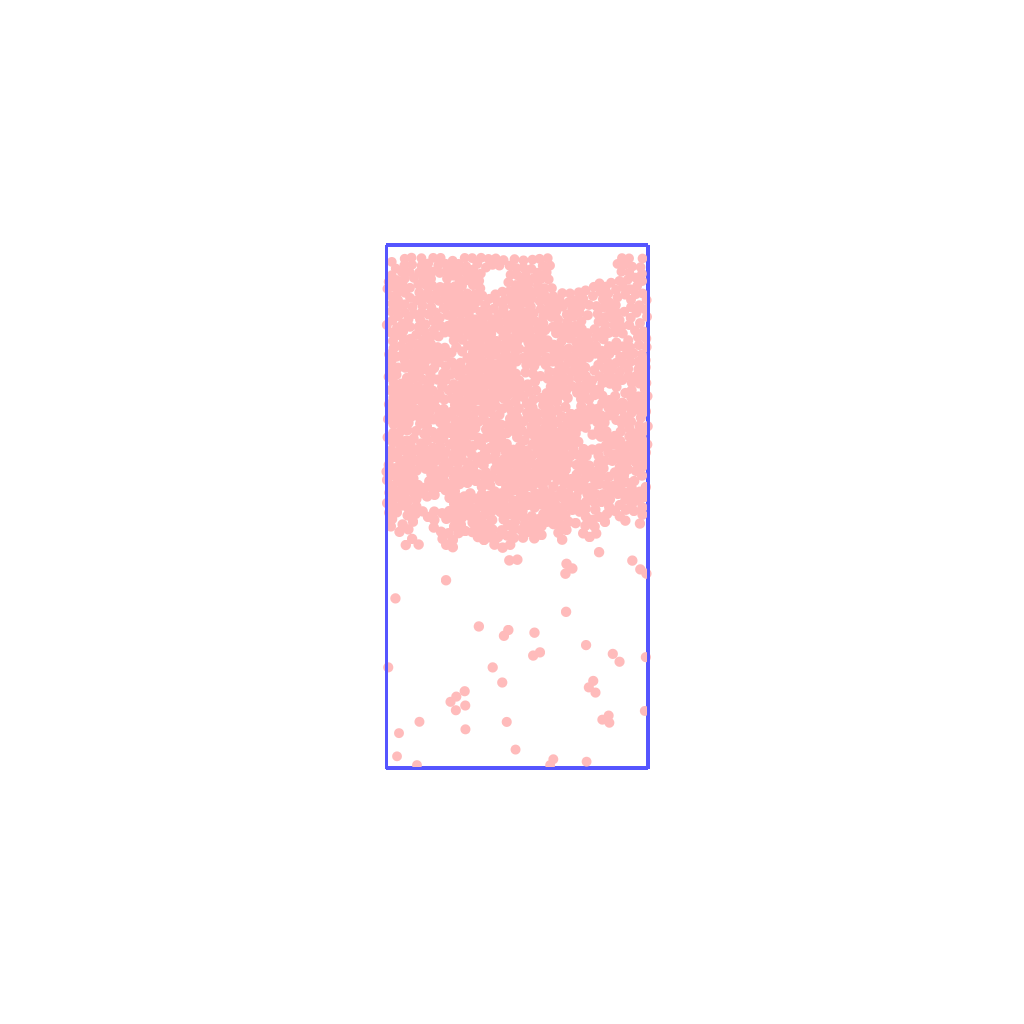
\includegraphics[width=\textwidth]{image/RaRtmap/2023-11-15T13:37:58.058__chi1.265_Ay50_rho0.4_T0.43_dT0.04_Rd0.0_Rt0.5_Ra0.938769_g0.0003999718779659611_run4.0e7_output.png}}
      \subcaption{$\text{R}_\text{a}=0.938,\\\text{R}_\text{t}=0.500$}
      % \label{}
    \end{minipage} &
    \begin{minipage}[t]{0.2\hsize}
      \centering
      \href{https://youtu.be/kSUk1XcKZBA}{
      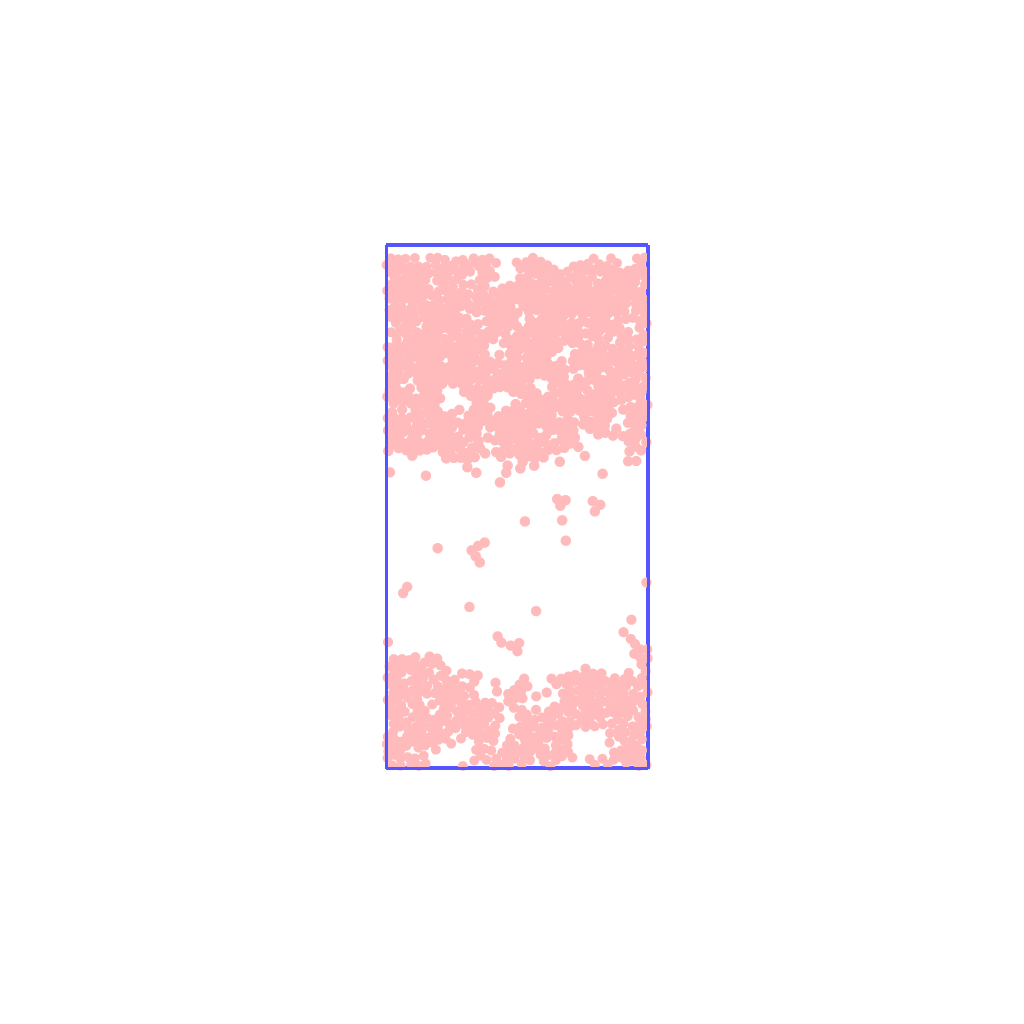
\includegraphics[width=\textwidth]{image/RaRtmap/2023-11-15T14:30:22.529__chi1.265_Ay50_rho0.4_T0.43_dT0.04_Rd0.0_Rt0.5_Ra1.4081535_g0.0003999718779659611_run4.0e7_output.png}}
      \subcaption{$\text{R}_\text{a}=1.408,\\\text{R}_\text{t}=0.500$}
      % \label{}
    \end{minipage} &
    \begin{minipage}[t]{0.2\hsize}
      \centering
      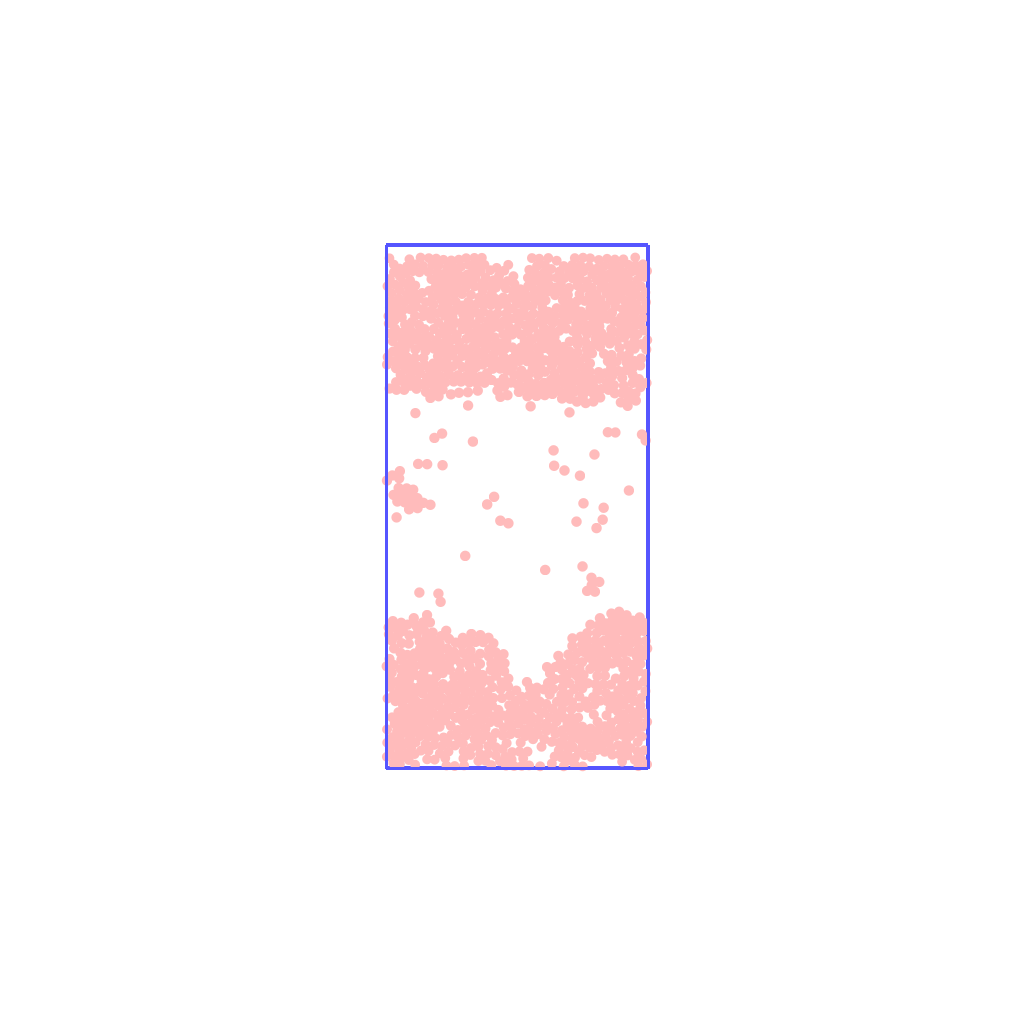
\includegraphics[width=\textwidth]{image/RaRtmap/2023-11-15T15:21:59.073__chi1.265_Ay50_rho0.4_T0.43_dT0.04_Rd0.0_Rt0.5_Ra1.877538_g0.0003999718779659611_run4.0e7_output.png}
      \subcaption{$\text{R}_\text{a}=1.877,\\\text{R}_\text{t}=0.500$}
      % \label{}
    \end{minipage} 
  \end{tabular}
  \caption{}
  % \lable{}
\end{figure}


重心位置$Y_g$を系の$y$幅でスケーリングして, 時系列プロットすると,

\begin{align}
  Y_g &\equiv \bar{y_i} = \frac{1}{N} \sum_{i}^{N} y_i
\end{align}

\begin{figure}[H]
  \begin{tabular}{ccccc}
    \begin{minipage}[t]{0.2\hsize}
      \centering
      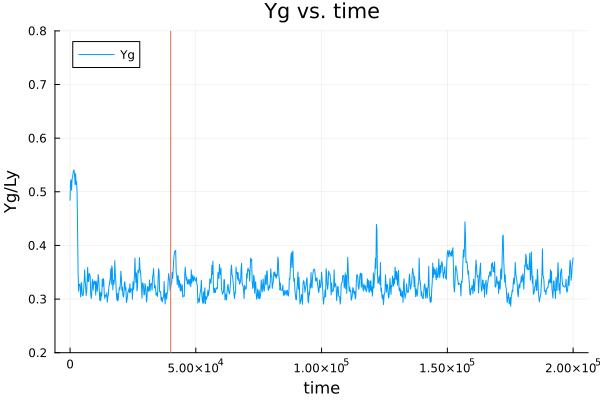
\includegraphics[width=\textwidth]{image/RaRtmap_time/2023-11-14T18:19:29.358__chi1.265_Ay50_rho0.4_T0.43_dT0.04_Rd0.0_Rt0.0_Ra0.0_g0.0003999718779659611_run4.0e7_output.png}
      \subcaption{$\text{R}_\text{a}=0.0,\\\text{R}_\text{t}=0.0$}
      \label{fig:RaRtmap_time_Ra0.0_Rt0.0}
    \end{minipage} &
    \begin{minipage}[t]{0.2\hsize}
      \centering
      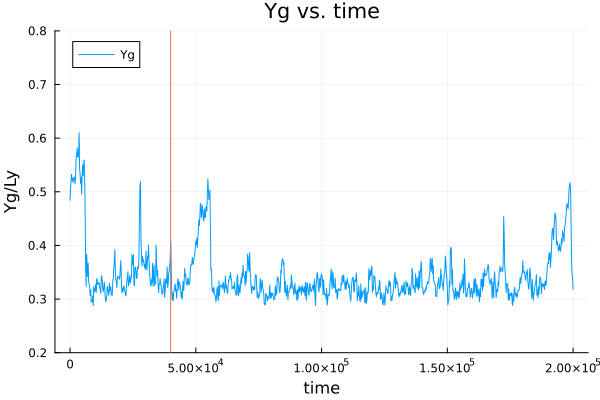
\includegraphics[width=\textwidth]{image/RaRtmap_time/2023-11-14T19:14:52.710__chi1.265_Ay50_rho0.4_T0.43_dT0.04_Rd0.0_Rt0.0_Ra0.4693845_g0.0003999718779659611_run4.0e7_output.png}
      \subcaption{$\text{R}_\text{a}=0.469,\\\text{R}_\text{t}=0.0$}
      \label{}
    \end{minipage} &
    \begin{minipage}[t]{0.2\hsize}
      \centering
      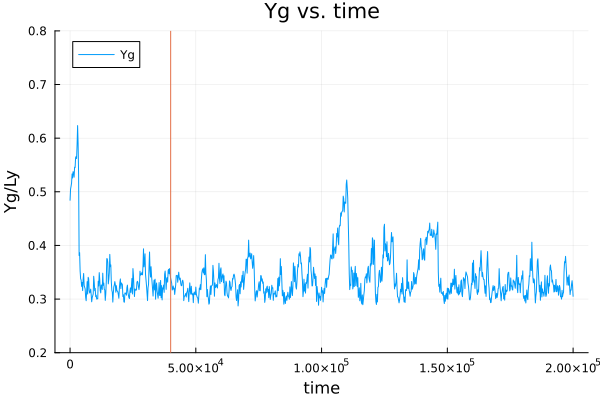
\includegraphics[width=\textwidth]{image/RaRtmap_time/2023-11-14T20:07:58.625__chi1.265_Ay50_rho0.4_T0.43_dT0.04_Rd0.0_Rt0.0_Ra0.938769_g0.0003999718779659611_run4.0e7_output.png}
      \subcaption{$\text{R}_\text{a}=0.938,\\\text{R}_\text{t}=0.0$}
      \label{}
    \end{minipage} &
    \begin{minipage}[t]{0.2\hsize}
      \centering
      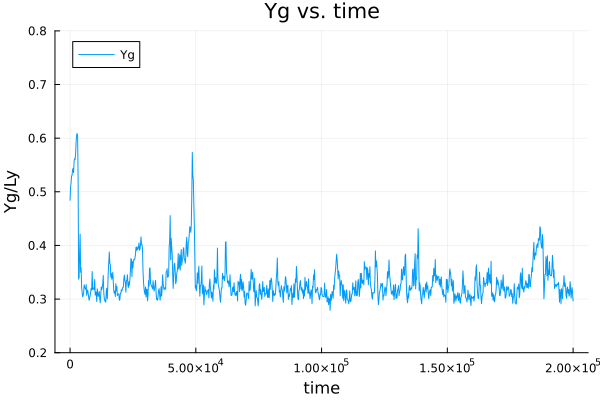
\includegraphics[width=\textwidth]{image/RaRtmap_time/2023-11-14T21:01:09.992__chi1.265_Ay50_rho0.4_T0.43_dT0.04_Rd0.0_Rt0.0_Ra1.4081535_g0.0003999718779659611_run4.0e7_output.png}
      \subcaption{$\text{R}_\text{a}=1.408,\\\text{R}_\text{t}=0.0$}
      \label{}
    \end{minipage} &
    \begin{minipage}[t]{0.2\hsize}
      \centering
      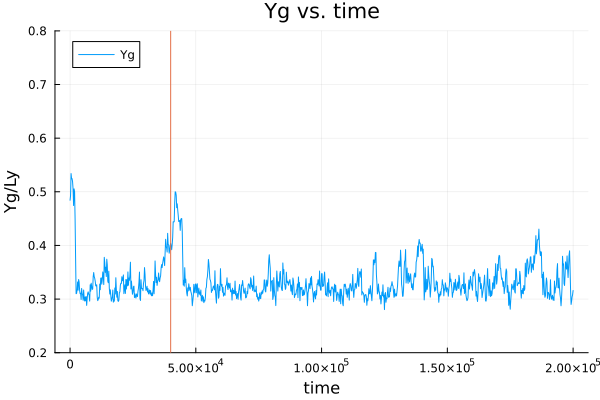
\includegraphics[width=\textwidth]{image/RaRtmap_time/2023-11-14T21:54:59.835__chi1.265_Ay50_rho0.4_T0.43_dT0.04_Rd0.0_Rt0.0_Ra1.877538_g0.0003999718779659611_run4.0e7_output.png}
      \subcaption{$\text{R}_\text{a}=1.877,\\\text{R}_\text{t}=0.0$}
      \label{}
    \end{minipage} \\
    \begin{minipage}[t]{0.2\hsize}
      \centering
      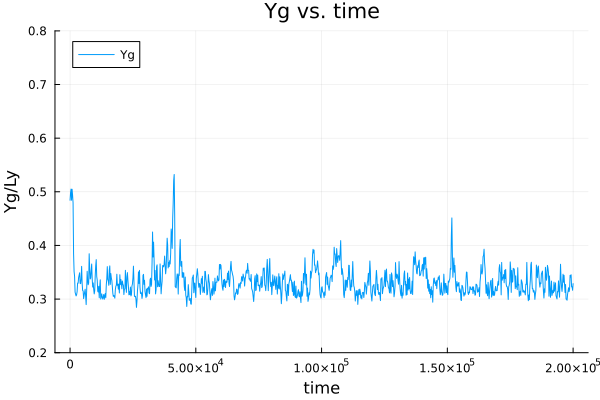
\includegraphics[width=\textwidth]{image/RaRtmap_time/2023-11-14T22:51:24.191__chi1.265_Ay50_rho0.4_T0.43_dT0.04_Rd0.0_Rt0.125_Ra0.0_g0.0003999718779659611_run4.0e7_output.png}
      \subcaption{$\text{R}_\text{a}=0.0,\\\text{R}_\text{t}=0.125$}
      \label{}
    \end{minipage} &
    \begin{minipage}[t]{0.2\hsize}
      \centering
      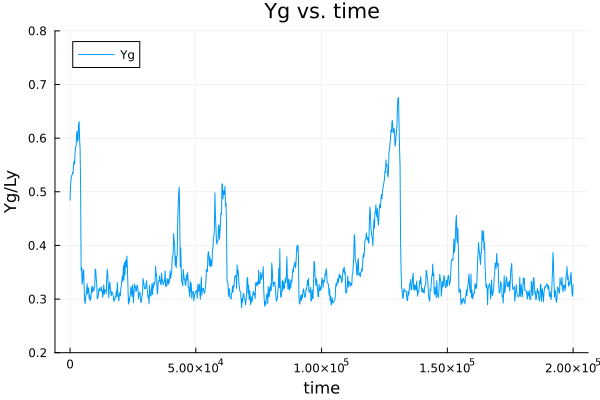
\includegraphics[width=\textwidth]{image/RaRtmap_time/2023-11-14T23:48:31.439__chi1.265_Ay50_rho0.4_T0.43_dT0.04_Rd0.0_Rt0.125_Ra0.4693845_g0.0003999718779659611_run4.0e7_output.png}
      \subcaption{$\text{R}_\text{a}=0.469,\\\text{R}_\text{t}=0.125$}
      \label{}
    \end{minipage} &
    \begin{minipage}[t]{0.2\hsize}
      \centering
      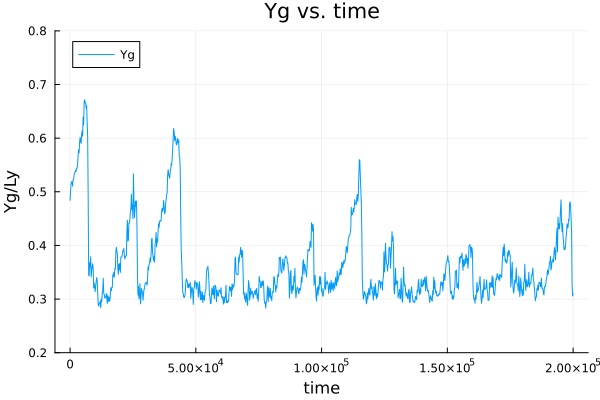
\includegraphics[width=\textwidth]{image/RaRtmap_time/2023-11-15T00:43:33.781__chi1.265_Ay50_rho0.4_T0.43_dT0.04_Rd0.0_Rt0.125_Ra0.938769_g0.0003999718779659611_run4.0e7_output.png}
      \subcaption{$\text{R}_\text{a}=0.938,\\\text{R}_\text{t}=0.125$}
      \label{}
    \end{minipage} &
    \begin{minipage}[t]{0.2\hsize}
      \centering
      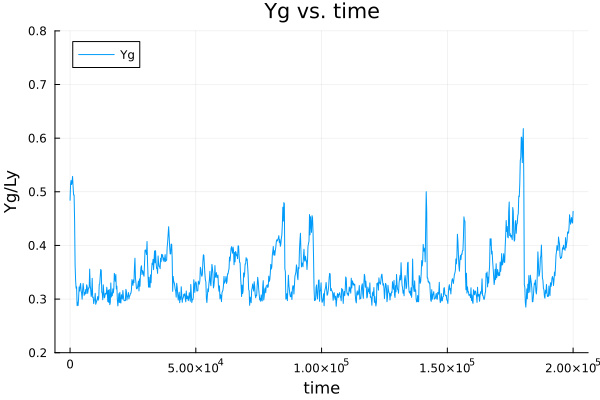
\includegraphics[width=\textwidth]{image/RaRtmap_time/2023-11-15T01:35:17.404__chi1.265_Ay50_rho0.4_T0.43_dT0.04_Rd0.0_Rt0.125_Ra1.4081535_g0.0003999718779659611_run4.0e7_output.png}
      \subcaption{$\text{R}_\text{a}=1.408,\\\text{R}_\text{t}=0.125$}
      \label{}
    \end{minipage} &
    \begin{minipage}[t]{0.2\hsize}
      \centering
      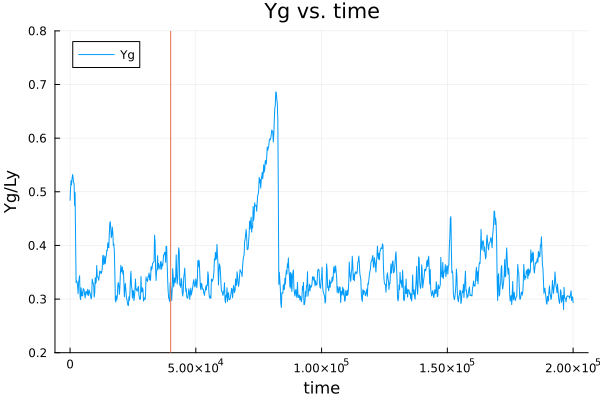
\includegraphics[width=\textwidth]{image/RaRtmap_time/2023-11-15T02:27:34.337__chi1.265_Ay50_rho0.4_T0.43_dT0.04_Rd0.0_Rt0.125_Ra1.877538_g0.0003999718779659611_run4.0e7_output.png}
      \subcaption{$\text{R}_\text{a}=1.877,\\\text{R}_\text{t}=0.125$}
      \label{}
    \end{minipage} \\
    \begin{minipage}[t]{0.2\hsize}
      \centering
      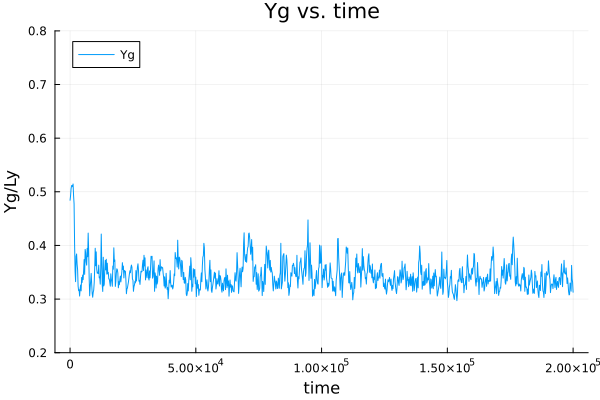
\includegraphics[width=\textwidth]{image/RaRtmap_time/2023-11-15T03:19:32.715__chi1.265_Ay50_rho0.4_T0.43_dT0.04_Rd0.0_Rt0.25_Ra0.0_g0.0003999718779659611_run4.0e7_output.png}
      \subcaption{$\text{R}_\text{a}=0.0,\\\text{R}_\text{t}=0.250$}
      \label{}
    \end{minipage} &
    \begin{minipage}[t]{0.2\hsize}
      \centering
      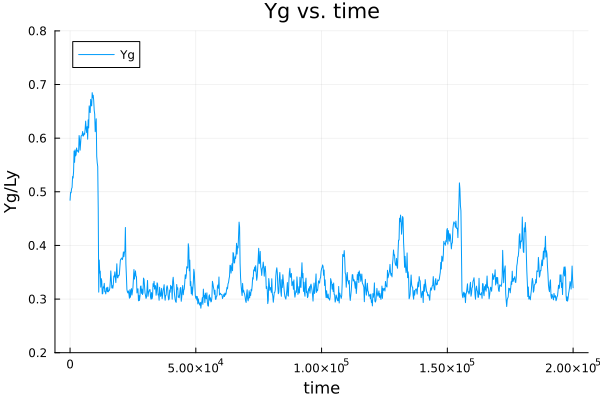
\includegraphics[width=\textwidth]{image/RaRtmap_time/2023-11-15T04:11:00.956__chi1.265_Ay50_rho0.4_T0.43_dT0.04_Rd0.0_Rt0.25_Ra0.4693845_g0.0003999718779659611_run4.0e7_output.png}
      \subcaption{$\text{R}_\text{a}=0.469,\\\text{R}_\text{t}=0.250$}
      \label{}
    \end{minipage} &
    \begin{minipage}[t]{0.2\hsize}
      \centering
      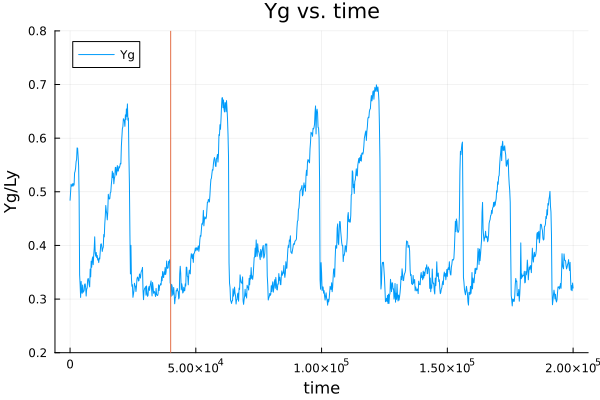
\includegraphics[width=\textwidth]{image/RaRtmap_time/2023-11-15T05:03:45.973__chi1.265_Ay50_rho0.4_T0.43_dT0.04_Rd0.0_Rt0.25_Ra0.938769_g0.0003999718779659611_run4.0e7_output.png}
      \subcaption{$\text{R}_\text{a}=0.938,\\\text{R}_\text{t}=0.250$}
      \label{}
    \end{minipage} &
    \begin{minipage}[t]{0.2\hsize}
      \centering
      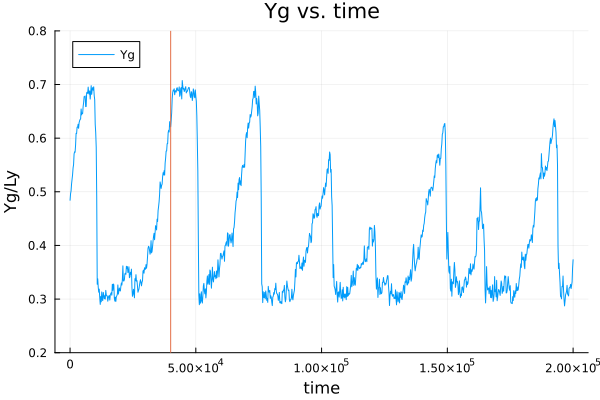
\includegraphics[width=\textwidth]{image/RaRtmap_time/2023-11-15T05:53:00.667__chi1.265_Ay50_rho0.4_T0.43_dT0.04_Rd0.0_Rt0.25_Ra1.4081535_g0.0003999718779659611_run4.0e7_output.png}
      \subcaption{$\text{R}_\text{a}=1.408,\\\text{R}_\text{t}=0.250$}
      \label{}
    \end{minipage} &
    \begin{minipage}[t]{0.2\hsize}
      \centering
      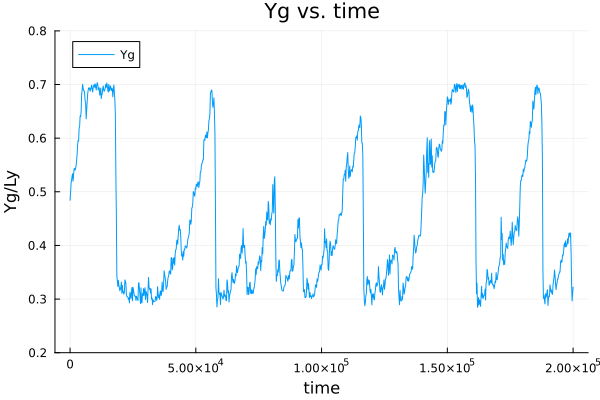
\includegraphics[width=\textwidth]{image/RaRtmap_time/2023-11-15T06:43:21.554__chi1.265_Ay50_rho0.4_T0.43_dT0.04_Rd0.0_Rt0.25_Ra1.877538_g0.0003999718779659611_run4.0e7_output.png}
      \subcaption{$\text{R}_\text{a}=1.877,\\\text{R}_\text{t}=0.250$}
      \label{}
    \end{minipage} \\
    \begin{minipage}[t]{0.2\hsize}
      \centering
      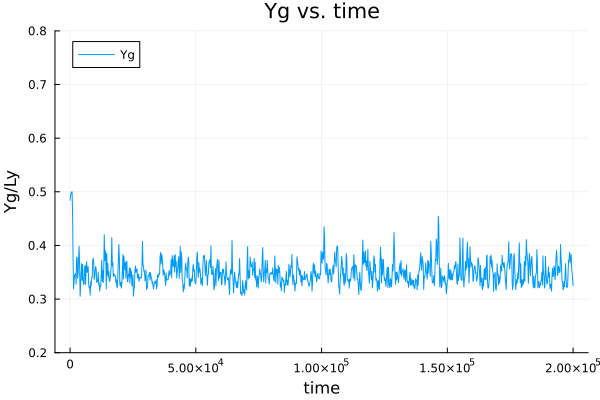
\includegraphics[width=\textwidth]{image/RaRtmap_time/2023-11-15T07:34:00.555__chi1.265_Ay50_rho0.4_T0.43_dT0.04_Rd0.0_Rt0.375_Ra0.0_g0.0003999718779659611_run4.0e7_output.png}
      \subcaption{$\text{R}_\text{a}=0.0,\\\text{R}_\text{t}=0.375$}
      \label{}
    \end{minipage} &
    \begin{minipage}[t]{0.2\hsize}
      \centering
      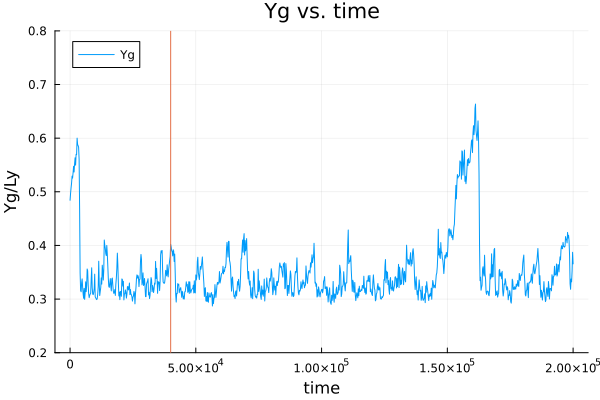
\includegraphics[width=\textwidth]{image/RaRtmap_time/2023-11-15T08:24:37.362__chi1.265_Ay50_rho0.4_T0.43_dT0.04_Rd0.0_Rt0.375_Ra0.4693845_g0.0003999718779659611_run4.0e7_output.png}
      \subcaption{$\text{R}_\text{a}=0.469,\\\text{R}_\text{t}=0.375$}
      \label{}
    \end{minipage} &
    \begin{minipage}[t]{0.2\hsize}
      \centering
      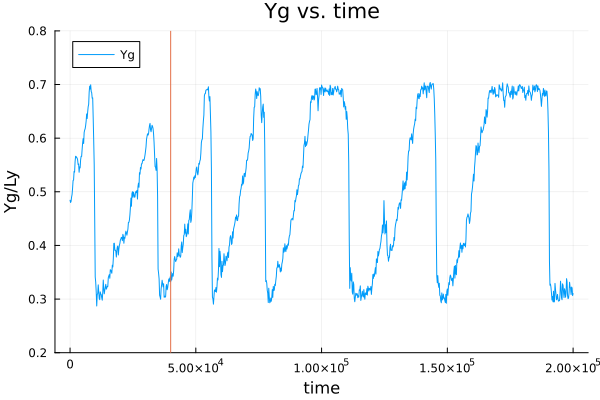
\includegraphics[width=\textwidth]{image/RaRtmap_time/2023-11-15T09:16:40.082__chi1.265_Ay50_rho0.4_T0.43_dT0.04_Rd0.0_Rt0.375_Ra0.938769_g0.0003999718779659611_run4.0e7_output.png}
      \subcaption{$\text{R}_\text{a}=0.938,\\\text{R}_\text{t}=0.375$}
      \label{}
    \end{minipage} &
    \begin{minipage}[t]{0.2\hsize}
      \centering
      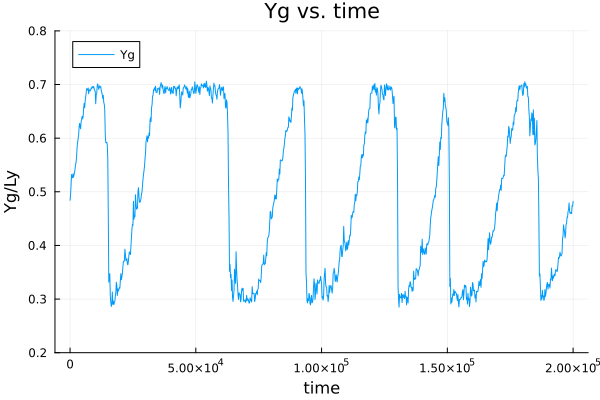
\includegraphics[width=\textwidth]{image/RaRtmap_time/2023-11-15T10:07:20.945__chi1.265_Ay50_rho0.4_T0.43_dT0.04_Rd0.0_Rt0.375_Ra1.4081535_g0.0003999718779659611_run4.0e7_output.png}
      \subcaption{$\text{R}_\text{a}=1.408,\\\text{R}_\text{t}=0.375$}
      \label{}
    \end{minipage} &
    \begin{minipage}[t]{0.2\hsize}
      \centering
      \includegraphics[width=\textwidth]{image/RaRtmap_time/2023-11-15T10:59:30.665__chi1.265_Ay50_rho0.4_T0.43_dT0.04_Rd0.0_Rt0.375_Ra1.877538_g0.0003999718779659611_run4.0e7_output.png}
      \subcaption{$\text{R}_\text{a}=1.877,\\\text{R}_\text{t}=0.375$}
      \label{}
    \end{minipage} \\
    \begin{minipage}[t]{0.2\hsize}
      \centering
      \includegraphics[width=\textwidth]{image/RaRtmap_time/2023-11-15T11:53:37.697__chi1.265_Ay50_rho0.4_T0.43_dT0.04_Rd0.0_Rt0.5_Ra0.0_g0.0003999718779659611_run4.0e7_output.png}
      \subcaption{$\text{R}_\text{a}=0.0,\\\text{R}_\text{t}=0.500$}
      \label{}
    \end{minipage} &
    \begin{minipage}[t]{0.2\hsize}
      \centering
      \includegraphics[width=\textwidth]{image/RaRtmap_time/2023-11-15T12:45:26.303__chi1.265_Ay50_rho0.4_T0.43_dT0.04_Rd0.0_Rt0.5_Ra0.4693845_g0.0003999718779659611_run4.0e7_output.png}
      \subcaption{$\text{R}_\text{a}=0.469,\\\text{R}_\text{t}=0.500$}
      \label{fig:RaRtmap_time_Ra0.469_Rt0.500}
    \end{minipage} &
    \begin{minipage}[t]{0.2\hsize}
      \centering
      \includegraphics[width=\textwidth]{image/RaRtmap_time/2023-11-15T13:37:58.058__chi1.265_Ay50_rho0.4_T0.43_dT0.04_Rd0.0_Rt0.5_Ra0.938769_g0.0003999718779659611_run4.0e7_output.png}
      \subcaption{$\text{R}_\text{a}=0.938,\\\text{R}_\text{t}=0.500$}
      \label{fig:RaRtmap_time_Ra0.938_Rt0.500}
    \end{minipage} &
    \begin{minipage}[t]{0.2\hsize}
      \centering
      \includegraphics[width=\textwidth]{image/RaRtmap_time/2023-11-15T14:30:22.529__chi1.265_Ay50_rho0.4_T0.43_dT0.04_Rd0.0_Rt0.5_Ra1.4081535_g0.0003999718779659611_run4.0e7_output.png}
      \subcaption{$\text{R}_\text{a}=1.408,\\\text{R}_\text{t}=0.500$}
      \label{}
    \end{minipage} &
    \begin{minipage}[t]{0.2\hsize}
      \centering
      \includegraphics[width=\textwidth]{image/RaRtmap_time/2023-11-15T15:21:59.073__chi1.265_Ay50_rho0.4_T0.43_dT0.04_Rd0.0_Rt0.5_Ra1.877538_g0.0003999718779659611_run4.0e7_output.png}
      \subcaption{$\text{R}_\text{a}=1.877,\\\text{R}_\text{t}=0.500$}
      \label{}
    \end{minipage} 
  \end{tabular}
  \caption{$t_i = 0, t_f = 2.0 \times 10^5, \dd t \sqrt{\varepsilon / m \sigma^2}= 0.005, t \sqrt{\varepsilon / m \sigma^2} = 200 ごとにプロット.$}
  \label{fig:RaRtmap_time}
\end{figure}


ここで, 重心の標準偏差は以下のように書くことができる.

\begin{align}
  \sigma (Y_g) &= \sqrt{\frac{1}{N_{D}}\sum_{t=t_i}^{t=t_f} (Y_{g}(t) - \bar{Y_g})^2}
\end{align}

重心位置の標準偏差について同時プロットで表してみる. 以降の解析は図\ref{fig:RaRtmap_time_Ra0.0_Rt0.0}から定常状態にあるとみなせる, $t_i \sqrt{\varepsilon / m \sigma^2} = 2.5 \times 10^{4}$からのデータを用いてプロットすることにしている.

\begin{figure}[H]
  \begin{tabular}{cc}
    \begin{minipage}[t]{0.5\hsize}
      \centering
      \includegraphics[width=\textwidth]{image/lnStdYg_Ra0.0to1.877538_Rt0.0to0.5_ti25000.png}
      \subcaption{}
      \label{}
    \end{minipage}
    \begin{minipage}[t]{0.5\hsize}
      \centering
      \includegraphics[width=\textwidth]{image/lnStdYg_Rt0.0to0.5_Ra0.0to1.877538_ti25000.png}
      \subcaption{}
      \label{}
    \end{minipage}
  \end{tabular}
  \caption{$t_i \sqrt{\varepsilon / m \sigma^2} = 2.5 \times 10^{4}$}
  \label{}
\end{figure}

\subsection{周期性}

重心位置が周期的に変化しているのかを調べたい.

図\ref{fig:RaRtmap_time_Ra0.469_Rt0.500}$R_a = 0.469, R_t = 0.5$と図\ref{fig:RaRtmap_time_Ra0.938_Rt0.500} $R_a = 0.938, R_t = 0.5$の間をもっと詳しく見る.

\begin{figure}[H]
  \centering
  \begin{tabular}{ccccc}
    \begin{minipage}[t]{0.2\hsize}
      \centering
      \includegraphics[width=\textwidth]{image/RaRtmap_time/2023-11-22T18:19:26.970_RaRt_chi1.265_Ay50_rho0.4_T0.43_dT0.04_Rd0.0_Rt0.5_Ra0.4693845_g0.0003999718779659611_run1.2e8.png}
      \subcaption{Ra0.4693845}
      \label{}
    \end{minipage} &
    \begin{minipage}[t]{0.2\hsize}
      \centering
      \includegraphics[width=\textwidth]{image/RaRtmap_time/2023-11-22T18:19:27.571_RaRt_chi1.265_Ay50_rho0.4_T0.43_dT0.04_Rd0.0_Rt0.5_Ra0.586730625_g0.0003999718779659611_run1.2e8.png}
      \subcaption{Ra0.586730625}
      \label{}
    \end{minipage} &
    \begin{minipage}[t]{0.2\hsize}
      \centering
      \includegraphics[width=\textwidth]{image/RaRtmap_time/2023-11-22T18:19:27.653_RaRt_chi1.265_Ay50_rho0.4_T0.43_dT0.04_Rd0.0_Rt0.5_Ra0.70407675_g0.0003999718779659611_run1.2e8.png}
      \subcaption{Ra0.70407675}
      \label{}
    \end{minipage} &
    \begin{minipage}[t]{0.2\hsize}
      \centering
      \includegraphics[width=\textwidth]{image/RaRtmap_time/2023-11-22T18:19:27.720_RaRt_chi1.265_Ay50_rho0.4_T0.43_dT0.04_Rd0.0_Rt0.5_Ra0.821422875_g0.0003999718779659611_run1.2e8.png}
      \subcaption{Ra0.821422875}
      \label{}
    \end{minipage} &
    \begin{minipage}[t]{0.2\hsize}
      \centering
      \includegraphics[width=\textwidth]{image/RaRtmap_time/2023-11-22T18:19:27.787_RaRt_chi1.265_Ay50_rho0.4_T0.43_dT0.04_Rd0.0_Rt0.5_Ra0.938769_g0.0003999718779659611_run1.2e8.png}
      \subcaption{Ra0.938769}
      \label{}
    \end{minipage} 
  \end{tabular}
  \caption{}
  \label{}
\end{figure}

\begin{figure}[H]
  \centering
  \includegraphics[scale=0.5]{image/lnStdYg_Ra0.4693845to0.98769_Rt0.5_ti25000.png}
  \caption{}
  \label{}
\end{figure}

% \begin{figure}[H]
%   \centering
%   \includegraphics[scale=0.6]{image/RaRtmap_time/2023-11-27T01:34:51.948_Ra_chi1.265_Ay50_rho0.4_T0.43_dT0.04_Rd0.0_Rt0.5_Ra0.70407675_g0.0003999718779659611_run1.2e9.png}
%   \caption{Ra0.4693845}
%   \label{}
% \end{figure}

\begin{figure}[H]
  \centering
  \begin{tabular}{ccccc}
    \begin{minipage}[t]{0.2\hsize}
      \centering
      \includegraphics[width=\textwidth]{image/RaRtmap_time/2023-11-27T01:34:51.948_Ra_chi1.265_Ay50_rho0.4_T0.43_dT0.04_Rd0.0_Rt0.5_Ra0.70407675_g0.0003999718779659611_run1.2e9.png}
      \subcaption{Ra0.70407675}
      \label{}
    \end{minipage} &
    \begin{minipage}[t]{0.2\hsize}
      \centering
      \includegraphics[width=\textwidth]{image/RaRtmap_time/2023-11-27T01:34:52.442_Ra_chi1.265_Ay50_rho0.4_T0.43_dT0.04_Rd0.0_Rt0.5_Ra0.7627498125_g0.0003999718779659611_run1.2e9.png}
      \subcaption{Ra0.7627498125}
      \label{}
    \end{minipage} &
    \begin{minipage}[t]{0.2\hsize}
      \centering
      \includegraphics[width=\textwidth]{image/RaRtmap_time/2023-11-27T01:34:52.545_Ra_chi1.265_Ay50_rho0.4_T0.43_dT0.04_Rd0.0_Rt0.5_Ra0.821422875_g0.0003999718779659611_run1.2e9.png}
      \subcaption{Ra0.821422875}
      \label{}
    \end{minipage} &
    \begin{minipage}[t]{0.2\hsize}
      \centering
      \includegraphics[width=\textwidth]{image/RaRtmap_time/2023-11-27T01:34:52.610_Ra_chi1.265_Ay50_rho0.4_T0.43_dT0.04_Rd0.0_Rt0.5_Ra0.8800959375_g0.0003999718779659611_run1.2e9.png}
      \subcaption{Ra0.8800959375}
      \label{}
    \end{minipage} &
    \begin{minipage}[t]{0.2\hsize}
      \centering
      \includegraphics[width=\textwidth]{image/RaRtmap_time/2023-11-27T01:34:52.675_Ra_chi1.265_Ay50_rho0.4_T0.43_dT0.04_Rd0.0_Rt0.5_Ra0.938769_g0.0003999718779659611_run1.2e9.png}
      \subcaption{Ra0.938769}
      \label{}
    \end{minipage} 
  \end{tabular}
  \caption{$t_i = 0 , t_f = 6.0 \times 10^6, t\sqrt{\epsilon/m{\sigma}^2} = 6000$ごとにプロット.}
  \label{}
\end{figure}

\begin{figure}[H]
  \centering
  \includegraphics[scale=0.5]{image/lnStdYg_Ra0.70407675to0.98769_Rt0.5_ti25000.png}
  \caption{}
  \label{}
\end{figure}

図\ref{fig:RaRtmap_time_Ra0.469_Rt0.500}$R_a = 0.469, R_t = 0.5$と図\ref{fig:RaRtmap_time_Ra0.938_Rt0.500} $R_a = 0.938, R_t = 0.5$の間をもっと詳しく見る. その際, 簡単のため, $Ra =0.5 \sim 1.0$の間を見ることにする.

\begin{figure}[H]
  \centering
  \begin{tabular}{ccccc}
    \begin{minipage}[t]{0.2\hsize}
      \centering
      \includegraphics[width=\textwidth]{image/RaRtmap_time/2023-11-30T20:13:31.872_Ra_chi1.265_Ay50_rho0.4_T0.43_dT0.04_Rd0.0_Rt0.5_Ra0.5_g0.0003999718779659611_run1.2e9.png}
      \subcaption{Ra0.5}
      \label{}
    \end{minipage} &
    \begin{minipage}[t]{0.2\hsize}
      \centering
      \includegraphics[width=\textwidth]{image/RaRtmap_time/2023-11-30T20:13:32.405_Ra_chi1.265_Ay50_rho0.4_T0.43_dT0.04_Rd0.0_Rt0.5_Ra0.625_g0.0003999718779659611_run1.2e9.png}
      \subcaption{Ra0.625}
      \label{}
    \end{minipage} &
    \begin{minipage}[t]{0.2\hsize}
      \centering
      \includegraphics[width=\textwidth]{image/RaRtmap_time/2023-11-30T20:13:32.471_Ra_chi1.265_Ay50_rho0.4_T0.43_dT0.04_Rd0.0_Rt0.5_Ra0.75_g0.0003999718779659611_run1.2e9.png}
      \subcaption{Ra0.75}
      \label{}
    \end{minipage} &
    \begin{minipage}[t]{0.2\hsize}
      \centering
      \includegraphics[width=\textwidth]{image/RaRtmap_time/2023-11-30T20:13:32.545_Ra_chi1.265_Ay50_rho0.4_T0.43_dT0.04_Rd0.0_Rt0.5_Ra0.875_g0.0003999718779659611_run1.2e9.png}
      \subcaption{Ra0.875}
      \label{}
    \end{minipage} &
    \begin{minipage}[t]{0.2\hsize}
      \centering
      \includegraphics[width=\textwidth]{image/RaRtmap_time/2023-11-30T20:13:32.620_Ra_chi1.265_Ay50_rho0.4_T0.43_dT0.04_Rd0.0_Rt0.5_Ra1.0_g0.0003999718779659611_run1.2e9.png}
      \subcaption{Ra1.0}
      \label{}
    \end{minipage} 
  \end{tabular}
  \caption{}
  \label{}
\end{figure}

\begin{figure}[H]
  \centering
  \includegraphics[scale=0.5]{image/lnStdYg_Ra0.5to1.0_Rt0.5_ti25000.png}
  \caption{}
  \label{}
\end{figure}

\subsection{サイクル}

図\ref{fig:RaRtmap_time}の結果をそれぞれ正規化したヒストグラムにして表す.

\begin{figure}[H]
  \begin{tabular}{ccccc}
    \begin{minipage}[t]{0.2\hsize}
      \centering
      \includegraphics[width=\textwidth]{image/RaRtmap_hist/2023-11-14T18:19:29.358__chi1.265_Ay50_rho0.4_T0.43_dT0.04_Rd0.0_Rt0.0_Ra0.0_g0.0003999718779659611_run4.0e7_output.png}
      \subcaption{$\text{R}_\text{a}=0.0,\text{R}_\text{t}=0.0$}
      \label{fig:RaRtmap_hist_Ra0.0_Rt0.0}
    \end{minipage} &
    \begin{minipage}[t]{0.2\hsize}
      \centering
      \includegraphics[width=\textwidth]{image/RaRtmap_hist/2023-11-14T19:14:52.710__chi1.265_Ay50_rho0.4_T0.43_dT0.04_Rd0.0_Rt0.0_Ra0.4693845_g0.0003999718779659611_run4.0e7_output.png}
      \subcaption{$\text{R}_\text{a}=0.469,\\\text{R}_\text{t}=0.0$}
      \label{}
    \end{minipage} &
    \begin{minipage}[t]{0.2\hsize}
      \centering
      \includegraphics[width=\textwidth]{image/RaRtmap_hist/2023-11-14T20:07:58.625__chi1.265_Ay50_rho0.4_T0.43_dT0.04_Rd0.0_Rt0.0_Ra0.938769_g0.0003999718779659611_run4.0e7_output.png}
      \subcaption{$\text{R}_\text{a}=0.938,\\\text{R}_\text{t}=0.0$}
      \label{}
    \end{minipage} &
    \begin{minipage}[t]{0.2\hsize}
      \centering
      \includegraphics[width=\textwidth]{image/RaRtmap_hist/2023-11-14T21:01:09.992__chi1.265_Ay50_rho0.4_T0.43_dT0.04_Rd0.0_Rt0.0_Ra1.4081535_g0.0003999718779659611_run4.0e7_output.png}
      \subcaption{$\text{R}_\text{a}=1.408,\\\text{R}_\text{t}=0.0$}
      \label{}
    \end{minipage} &
    \begin{minipage}[t]{0.2\hsize}
      \centering
      \includegraphics[width=\textwidth]{image/RaRtmap_hist/2023-11-14T21:54:59.835__chi1.265_Ay50_rho0.4_T0.43_dT0.04_Rd0.0_Rt0.0_Ra1.877538_g0.0003999718779659611_run4.0e7_output.png}
      \subcaption{$\text{R}_\text{a}=1.877,\\\text{R}_\text{t}=0.0$}
      \label{}
    \end{minipage} \\
    \begin{minipage}[t]{0.2\hsize}
      \centering
      \includegraphics[width=\textwidth]{image/RaRtmap_hist/2023-11-14T22:51:24.191__chi1.265_Ay50_rho0.4_T0.43_dT0.04_Rd0.0_Rt0.125_Ra0.0_g0.0003999718779659611_run4.0e7_output.png}
      \subcaption{$\text{R}_\text{a}=0.0,\\\text{R}_\text{t}=0.125$}
      \label{}
    \end{minipage} &
    \begin{minipage}[t]{0.2\hsize}
      \centering
      \includegraphics[width=\textwidth]{image/RaRtmap_hist/2023-11-14T23:48:31.439__chi1.265_Ay50_rho0.4_T0.43_dT0.04_Rd0.0_Rt0.125_Ra0.4693845_g0.0003999718779659611_run4.0e7_output.png}
      \subcaption{$\text{R}_\text{a}=0.469,\\\text{R}_\text{t}=0.125$}
      \label{}
    \end{minipage} &
    \begin{minipage}[t]{0.2\hsize}
      \centering
      \includegraphics[width=\textwidth]{image/RaRtmap_hist/2023-11-15T00:43:33.781__chi1.265_Ay50_rho0.4_T0.43_dT0.04_Rd0.0_Rt0.125_Ra0.938769_g0.0003999718779659611_run4.0e7_output.png}
      \subcaption{$\text{R}_\text{a}=0.938,\\\text{R}_\text{t}=0.125$}
      \label{}
    \end{minipage} &
    \begin{minipage}[t]{0.2\hsize}
      \centering
      \includegraphics[width=\textwidth]{image/RaRtmap_hist/2023-11-15T01:35:17.404__chi1.265_Ay50_rho0.4_T0.43_dT0.04_Rd0.0_Rt0.125_Ra1.4081535_g0.0003999718779659611_run4.0e7_output.png}
      \subcaption{$\text{R}_\text{a}=1.408,\\\text{R}_\text{t}=0.125$}
      \label{}
    \end{minipage} &
    \begin{minipage}[t]{0.2\hsize}
      \centering
      \includegraphics[width=\textwidth]{image/RaRtmap_hist/2023-11-15T02:27:34.337__chi1.265_Ay50_rho0.4_T0.43_dT0.04_Rd0.0_Rt0.125_Ra1.877538_g0.0003999718779659611_run4.0e7_output.png}
      \subcaption{$\text{R}_\text{a}=1.877,\\\text{R}_\text{t}=0.125$}
      \label{}
    \end{minipage} \\
    \begin{minipage}[t]{0.2\hsize}
      \centering
      \includegraphics[width=\textwidth]{image/RaRtmap_hist/2023-11-15T03:19:32.715__chi1.265_Ay50_rho0.4_T0.43_dT0.04_Rd0.0_Rt0.25_Ra0.0_g0.0003999718779659611_run4.0e7_output.png}
      \subcaption{$\text{R}_\text{a}=0.0,\\\text{R}_\text{t}=0.250$}
      \label{}
    \end{minipage} &
    \begin{minipage}[t]{0.2\hsize}
      \centering
      \includegraphics[width=\textwidth]{image/RaRtmap_hist/2023-11-15T04:11:00.956__chi1.265_Ay50_rho0.4_T0.43_dT0.04_Rd0.0_Rt0.25_Ra0.4693845_g0.0003999718779659611_run4.0e7_output.png}
      \subcaption{$\text{R}_\text{a}=0.469,\\\text{R}_\text{t}=0.250$}
      \label{}
    \end{minipage} &
    \begin{minipage}[t]{0.2\hsize}
      \centering
      \includegraphics[width=\textwidth]{image/RaRtmap_hist/2023-11-15T05:03:45.973__chi1.265_Ay50_rho0.4_T0.43_dT0.04_Rd0.0_Rt0.25_Ra0.938769_g0.0003999718779659611_run4.0e7_output.png}
      \subcaption{$\text{R}_\text{a}=0.938,\\\text{R}_\text{t}=0.250$}
      \label{}
    \end{minipage} &
    \begin{minipage}[t]{0.2\hsize}
      \centering
      \includegraphics[width=\textwidth]{image/RaRtmap_hist/2023-11-15T05:53:00.667__chi1.265_Ay50_rho0.4_T0.43_dT0.04_Rd0.0_Rt0.25_Ra1.4081535_g0.0003999718779659611_run4.0e7_output.png}
      \subcaption{$\text{R}_\text{a}=1.408,\\\text{R}_\text{t}=0.250$}
      \label{}
    \end{minipage} &
    \begin{minipage}[t]{0.2\hsize}
      \centering
      \includegraphics[width=\textwidth]{image/RaRtmap_hist/2023-11-15T06:43:21.554__chi1.265_Ay50_rho0.4_T0.43_dT0.04_Rd0.0_Rt0.25_Ra1.877538_g0.0003999718779659611_run4.0e7_output.png}
      \subcaption{$\text{R}_\text{a}=1.877,\\\text{R}_\text{t}=0.250$}
      \label{}
    \end{minipage} \\
    \begin{minipage}[t]{0.2\hsize}
      \centering
      \includegraphics[width=\textwidth]{image/RaRtmap_hist/2023-11-15T07:34:00.555__chi1.265_Ay50_rho0.4_T0.43_dT0.04_Rd0.0_Rt0.375_Ra0.0_g0.0003999718779659611_run4.0e7_output.png}
      \subcaption{$\text{R}_\text{a}=0.0,\\\text{R}_\text{t}=0.375$}
      \label{}
    \end{minipage} &
    \begin{minipage}[t]{0.2\hsize}
      \centering
      \includegraphics[width=\textwidth]{image/RaRtmap_hist/2023-11-15T08:24:37.362__chi1.265_Ay50_rho0.4_T0.43_dT0.04_Rd0.0_Rt0.375_Ra0.4693845_g0.0003999718779659611_run4.0e7_output.png}
      \subcaption{$\text{R}_\text{a}=0.469,\\\text{R}_\text{t}=0.375$}
      \label{}
    \end{minipage} &
    \begin{minipage}[t]{0.2\hsize}
      \centering
      \includegraphics[width=\textwidth]{image/RaRtmap_hist/2023-11-15T09:16:40.082__chi1.265_Ay50_rho0.4_T0.43_dT0.04_Rd0.0_Rt0.375_Ra0.938769_g0.0003999718779659611_run4.0e7_output.png}
      \subcaption{$\text{R}_\text{a}=0.938,\\\text{R}_\text{t}=0.375$}
      \label{}
    \end{minipage} &
    \begin{minipage}[t]{0.2\hsize}
      \centering
      \includegraphics[width=\textwidth]{image/RaRtmap_hist/2023-11-15T10:07:20.945__chi1.265_Ay50_rho0.4_T0.43_dT0.04_Rd0.0_Rt0.375_Ra1.4081535_g0.0003999718779659611_run4.0e7_output.png}
      \subcaption{$\text{R}_\text{a}=1.408,\\\text{R}_\text{t}=0.375$}
      \label{}
    \end{minipage} &
    \begin{minipage}[t]{0.2\hsize}
      \centering
      \includegraphics[width=\textwidth]{image/RaRtmap_hist/2023-11-15T10:59:30.665__chi1.265_Ay50_rho0.4_T0.43_dT0.04_Rd0.0_Rt0.375_Ra1.877538_g0.0003999718779659611_run4.0e7_output.png}
      \subcaption{$\text{R}_\text{a}=1.877,\\\text{R}_\text{t}=0.375$}
      \label{}
    \end{minipage} \\
    \begin{minipage}[t]{0.2\hsize}
      \centering
      \includegraphics[width=\textwidth]{image/RaRtmap_hist/2023-11-15T11:53:37.697__chi1.265_Ay50_rho0.4_T0.43_dT0.04_Rd0.0_Rt0.5_Ra0.0_g0.0003999718779659611_run4.0e7_output.png}
      \subcaption{$\text{R}_\text{a}=0.0,\\\text{R}_\text{t}=0.500$}
      \label{}
    \end{minipage} &
    \begin{minipage}[t]{0.2\hsize}
      \centering
      \includegraphics[width=\textwidth]{image/RaRtmap_hist/2023-11-15T12:45:26.303__chi1.265_Ay50_rho0.4_T0.43_dT0.04_Rd0.0_Rt0.5_Ra0.4693845_g0.0003999718779659611_run4.0e7_output.png}
      \subcaption{$\text{R}_\text{a}=0.469,\\\text{R}_\text{t}=0.500$}
      \label{fig:RaRtmap_hist_Ra0.469_Rt0.500}
    \end{minipage} &
    \begin{minipage}[t]{0.2\hsize}
      \centering
      \includegraphics[width=\textwidth]{image/RaRtmap_hist/2023-11-15T13:37:58.058__chi1.265_Ay50_rho0.4_T0.43_dT0.04_Rd0.0_Rt0.5_Ra0.938769_g0.0003999718779659611_run4.0e7_output.png}
      \subcaption{$\text{R}_\text{a}=0.938,\\\text{R}_\text{t}=0.500$}
      \label{fig:RaRtmap_hist_Ra0.938_Rt0.500}
    \end{minipage} &
    \begin{minipage}[t]{0.2\hsize}
      \centering
      \includegraphics[width=\textwidth]{image/RaRtmap_hist/2023-11-15T14:30:22.529__chi1.265_Ay50_rho0.4_T0.43_dT0.04_Rd0.0_Rt0.5_Ra1.4081535_g0.0003999718779659611_run4.0e7_output.png}
      \subcaption{$\text{R}_\text{a}=1.408,\\\text{R}_\text{t}=0.500$}
      \label{}
    \end{minipage} &
    \begin{minipage}[t]{0.2\hsize}
      \centering
      \includegraphics[width=\textwidth]{image/RaRtmap_hist/2023-11-15T15:21:59.073__chi1.265_Ay50_rho0.4_T0.43_dT0.04_Rd0.0_Rt0.5_Ra1.877538_g0.0003999718779659611_run4.0e7_output.png}
      \subcaption{$\text{R}_\text{a}=1.877,\\\text{R}_\text{t}=0.500$}
      \label{}
    \end{minipage} 
  \end{tabular}
  \caption{$t_i = 0, t_f = 2.0 \times 10^5, \dd t \sqrt{\varepsilon / m \sigma^2}= 0.005, t \sqrt{\varepsilon / m \sigma^2} = 200 ごとにY_g をプロットしたもののヒストグラム. ビン数は共通で50本.$}
  \label{}
\end{figure}


粒子集団のばらつき具合を時系列で考える.

\begin{align}
  \sigma_{y} (t)
  &= \sqrt{\frac{1}{N} \sum_{i=1}^{N} (y_i (t) - \bar{y_i}(t) )^2} \\
  &= \sqrt{\frac{1}{N} \sum_{i=1}^{N} (y_i (t) - Y_g (t) )^2} \\
  &= \sqrt{\frac{1}{N} \sum_{i=1}^{N} {{y_i} (t)}^2 - {{Y_g} (t)}^2}
\end{align}

\begin{figure}[H]
  \begin{tabular}{ccccc}
    \begin{minipage}[t]{0.2\hsize}
      \centering
      \includegraphics[width=\textwidth]{image/RaRtmap_cycle/2023-11-14T18:19:29.358__chi1.265_Ay50_rho0.4_T0.43_dT0.04_Rd0.0_Rt0.0_Ra0.0_g0.0003999718779659611_run4.0e7_output.png}
      \subcaption{$\text{R}_\text{a}=0.0,\text{R}_\text{t}=0.0$}
      \label{fig:RaRtmap_cycle_Ra0.0_Rt0.0}
    \end{minipage} &
    \begin{minipage}[t]{0.2\hsize}
      \centering
      \includegraphics[width=\textwidth]{image/RaRtmap_cycle/2023-11-14T19:14:52.710__chi1.265_Ay50_rho0.4_T0.43_dT0.04_Rd0.0_Rt0.0_Ra0.4693845_g0.0003999718779659611_run4.0e7_output.png}
      \subcaption{$\text{R}_\text{a}=0.469,\\\text{R}_\text{t}=0.0$}
      \label{}
    \end{minipage} &
    \begin{minipage}[t]{0.2\hsize}
      \centering
      \includegraphics[width=\textwidth]{image/RaRtmap_cycle/2023-11-14T20:07:58.625__chi1.265_Ay50_rho0.4_T0.43_dT0.04_Rd0.0_Rt0.0_Ra0.938769_g0.0003999718779659611_run4.0e7_output.png}
      \subcaption{$\text{R}_\text{a}=0.938,\\\text{R}_\text{t}=0.0$}
      \label{}
    \end{minipage} &
    \begin{minipage}[t]{0.2\hsize}
      \centering
      \includegraphics[width=\textwidth]{image/RaRtmap_cycle/2023-11-14T21:01:09.992__chi1.265_Ay50_rho0.4_T0.43_dT0.04_Rd0.0_Rt0.0_Ra1.4081535_g0.0003999718779659611_run4.0e7_output.png}
      \subcaption{$\text{R}_\text{a}=1.408,\\\text{R}_\text{t}=0.0$}
      \label{}
    \end{minipage} &
    \begin{minipage}[t]{0.2\hsize}
      \centering
      \includegraphics[width=\textwidth]{image/RaRtmap_cycle/2023-11-14T21:54:59.835__chi1.265_Ay50_rho0.4_T0.43_dT0.04_Rd0.0_Rt0.0_Ra1.877538_g0.0003999718779659611_run4.0e7_output.png}
      \subcaption{$\text{R}_\text{a}=1.877,\\\text{R}_\text{t}=0.0$}
      \label{}
    \end{minipage} \\
    \begin{minipage}[t]{0.2\hsize}
      \centering
      \includegraphics[width=\textwidth]{image/RaRtmap_cycle/2023-11-14T22:51:24.191__chi1.265_Ay50_rho0.4_T0.43_dT0.04_Rd0.0_Rt0.125_Ra0.0_g0.0003999718779659611_run4.0e7_output.png}
      \subcaption{$\text{R}_\text{a}=0.0,\\\text{R}_\text{t}=0.125$}
      \label{}
    \end{minipage} &
    \begin{minipage}[t]{0.2\hsize}
      \centering
      \includegraphics[width=\textwidth]{image/RaRtmap_cycle/2023-11-14T23:48:31.439__chi1.265_Ay50_rho0.4_T0.43_dT0.04_Rd0.0_Rt0.125_Ra0.4693845_g0.0003999718779659611_run4.0e7_output.png}
      \subcaption{$\text{R}_\text{a}=0.469,\\\text{R}_\text{t}=0.125$}
      \label{}
    \end{minipage} &
    \begin{minipage}[t]{0.2\hsize}
      \centering
      \includegraphics[width=\textwidth]{image/RaRtmap_cycle/2023-11-15T00:43:33.781__chi1.265_Ay50_rho0.4_T0.43_dT0.04_Rd0.0_Rt0.125_Ra0.938769_g0.0003999718779659611_run4.0e7_output.png}
      \subcaption{$\text{R}_\text{a}=0.938,\\\text{R}_\text{t}=0.125$}
      \label{}
    \end{minipage} &
    \begin{minipage}[t]{0.2\hsize}
      \centering
      \includegraphics[width=\textwidth]{image/RaRtmap_cycle/2023-11-15T01:35:17.404__chi1.265_Ay50_rho0.4_T0.43_dT0.04_Rd0.0_Rt0.125_Ra1.4081535_g0.0003999718779659611_run4.0e7_output.png}
      \subcaption{$\text{R}_\text{a}=1.408,\\\text{R}_\text{t}=0.125$}
      \label{}
    \end{minipage} &
    \begin{minipage}[t]{0.2\hsize}
      \centering
      \includegraphics[width=\textwidth]{image/RaRtmap_cycle/2023-11-15T02:27:34.337__chi1.265_Ay50_rho0.4_T0.43_dT0.04_Rd0.0_Rt0.125_Ra1.877538_g0.0003999718779659611_run4.0e7_output.png}
      \subcaption{$\text{R}_\text{a}=1.877,\\\text{R}_\text{t}=0.125$}
      \label{}
    \end{minipage} \\
    \begin{minipage}[t]{0.2\hsize}
      \centering
      \includegraphics[width=\textwidth]{image/RaRtmap_cycle/2023-11-15T03:19:32.715__chi1.265_Ay50_rho0.4_T0.43_dT0.04_Rd0.0_Rt0.25_Ra0.0_g0.0003999718779659611_run4.0e7_output.png}
      \subcaption{$\text{R}_\text{a}=0.0,\\\text{R}_\text{t}=0.250$}
      \label{}
    \end{minipage} &
    \begin{minipage}[t]{0.2\hsize}
      \centering
      \includegraphics[width=\textwidth]{image/RaRtmap_cycle/2023-11-15T04:11:00.956__chi1.265_Ay50_rho0.4_T0.43_dT0.04_Rd0.0_Rt0.25_Ra0.4693845_g0.0003999718779659611_run4.0e7_output.png}
      \subcaption{$\text{R}_\text{a}=0.469,\\\text{R}_\text{t}=0.250$}
      \label{}
    \end{minipage} &
    \begin{minipage}[t]{0.2\hsize}
      \centering
      \includegraphics[width=\textwidth]{image/RaRtmap_cycle/2023-11-15T05:03:45.973__chi1.265_Ay50_rho0.4_T0.43_dT0.04_Rd0.0_Rt0.25_Ra0.938769_g0.0003999718779659611_run4.0e7_output.png}
      \subcaption{$\text{R}_\text{a}=0.938,\\\text{R}_\text{t}=0.250$}
      \label{}
    \end{minipage} &
    \begin{minipage}[t]{0.2\hsize}
      \centering
      \includegraphics[width=\textwidth]{image/RaRtmap_cycle/2023-11-15T05:53:00.667__chi1.265_Ay50_rho0.4_T0.43_dT0.04_Rd0.0_Rt0.25_Ra1.4081535_g0.0003999718779659611_run4.0e7_output.png}
      \subcaption{$\text{R}_\text{a}=1.408,\\\text{R}_\text{t}=0.250$}
      \label{}
    \end{minipage} &
    \begin{minipage}[t]{0.2\hsize}
      \centering
      \includegraphics[width=\textwidth]{image/RaRtmap_cycle/2023-11-15T06:43:21.554__chi1.265_Ay50_rho0.4_T0.43_dT0.04_Rd0.0_Rt0.25_Ra1.877538_g0.0003999718779659611_run4.0e7_output.png}
      \subcaption{$\text{R}_\text{a}=1.877,\\\text{R}_\text{t}=0.250$}
      \label{}
    \end{minipage} \\
    \begin{minipage}[t]{0.2\hsize}
      \centering
      \includegraphics[width=\textwidth]{image/RaRtmap_cycle/2023-11-15T07:34:00.555__chi1.265_Ay50_rho0.4_T0.43_dT0.04_Rd0.0_Rt0.375_Ra0.0_g0.0003999718779659611_run4.0e7_output.png}
      \subcaption{$\text{R}_\text{a}=0.0,\\\text{R}_\text{t}=0.375$}
      \label{}
    \end{minipage} &
    \begin{minipage}[t]{0.2\hsize}
      \centering
      \includegraphics[width=\textwidth]{image/RaRtmap_cycle/2023-11-15T08:24:37.362__chi1.265_Ay50_rho0.4_T0.43_dT0.04_Rd0.0_Rt0.375_Ra0.4693845_g0.0003999718779659611_run4.0e7_output.png}
      \subcaption{$\text{R}_\text{a}=0.469,\\\text{R}_\text{t}=0.375$}
      \label{}
    \end{minipage} &
    \begin{minipage}[t]{0.2\hsize}
      \centering
      \includegraphics[width=\textwidth]{image/RaRtmap_cycle/2023-11-15T09:16:40.082__chi1.265_Ay50_rho0.4_T0.43_dT0.04_Rd0.0_Rt0.375_Ra0.938769_g0.0003999718779659611_run4.0e7_output.png}
      \subcaption{$\text{R}_\text{a}=0.938,\\\text{R}_\text{t}=0.375$}
      \label{}
    \end{minipage} &
    \begin{minipage}[t]{0.2\hsize}
      \centering
      \includegraphics[width=\textwidth]{image/RaRtmap_cycle/2023-11-15T10:07:20.945__chi1.265_Ay50_rho0.4_T0.43_dT0.04_Rd0.0_Rt0.375_Ra1.4081535_g0.0003999718779659611_run4.0e7_output.png}
      \subcaption{$\text{R}_\text{a}=1.408,\\\text{R}_\text{t}=0.375$}
      \label{}
    \end{minipage} &
    \begin{minipage}[t]{0.2\hsize}
      \centering
      \includegraphics[width=\textwidth]{image/RaRtmap_cycle/2023-11-15T10:59:30.665__chi1.265_Ay50_rho0.4_T0.43_dT0.04_Rd0.0_Rt0.375_Ra1.877538_g0.0003999718779659611_run4.0e7_output.png}
      \subcaption{$\text{R}_\text{a}=1.877,\\\text{R}_\text{t}=0.375$}
      \label{}
    \end{minipage} \\
    \begin{minipage}[t]{0.2\hsize}
      \centering
      \includegraphics[width=\textwidth]{image/RaRtmap_cycle/2023-11-15T11:53:37.697__chi1.265_Ay50_rho0.4_T0.43_dT0.04_Rd0.0_Rt0.5_Ra0.0_g0.0003999718779659611_run4.0e7_output.png}
      \subcaption{$\text{R}_\text{a}=0.0,\\\text{R}_\text{t}=0.500$}
      \label{}
    \end{minipage} &
    \begin{minipage}[t]{0.2\hsize}
      \centering
      \includegraphics[width=\textwidth]{image/RaRtmap_cycle/2023-11-15T12:45:26.303__chi1.265_Ay50_rho0.4_T0.43_dT0.04_Rd0.0_Rt0.5_Ra0.4693845_g0.0003999718779659611_run4.0e7_output.png}
      \subcaption{$\text{R}_\text{a}=0.469,\\\text{R}_\text{t}=0.500$}
      \label{fig:RaRtmap_cycle_Ra0.469_Rt0.500}
    \end{minipage} &
    \begin{minipage}[t]{0.2\hsize}
      \centering
      \includegraphics[width=\textwidth]{image/RaRtmap_cycle/2023-11-15T13:37:58.058__chi1.265_Ay50_rho0.4_T0.43_dT0.04_Rd0.0_Rt0.5_Ra0.938769_g0.0003999718779659611_run4.0e7_output.png}
      \subcaption{$\text{R}_\text{a}=0.938,\\\text{R}_\text{t}=0.500$}
      \label{fig:RaRtmap_cycle_Ra0.938_Rt0.500}
    \end{minipage} &
    \begin{minipage}[t]{0.2\hsize}
      \centering
      \includegraphics[width=\textwidth]{image/RaRtmap_cycle/2023-11-15T14:30:22.529__chi1.265_Ay50_rho0.4_T0.43_dT0.04_Rd0.0_Rt0.5_Ra1.4081535_g0.0003999718779659611_run4.0e7_output.png}
      \subcaption{$\text{R}_\text{a}=1.408,\\\text{R}_\text{t}=0.500$}
      \label{}
    \end{minipage} &
    \begin{minipage}[t]{0.2\hsize}
      \centering
      \includegraphics[width=\textwidth]{image/RaRtmap_cycle/2023-11-15T15:21:59.073__chi1.265_Ay50_rho0.4_T0.43_dT0.04_Rd0.0_Rt0.5_Ra1.877538_g0.0003999718779659611_run4.0e7_output.png}
      \subcaption{$\text{R}_\text{a}=1.877,\\\text{R}_\text{t}=0.500$}
      \label{}
    \end{minipage} 
  \end{tabular}
  \caption{$t_i = 4.0 \times 10^4, t_f = 2.0 \times 10^5, \dd t \sqrt{\varepsilon / m \sigma^2}= 0.005, t \sqrt{\varepsilon / m \sigma^2} = 200 ごとにプロット.$}
  \label{}
\end{figure}


\begin{figure}[H]
  \begin{tabular}{ccccc}
    \begin{minipage}[t]{0.2\hsize}
      \centering
      \includegraphics[width=\textwidth]{image/RaRtmap_cycle3d/2023-11-14T18:19:29.358__chi1.265_Ay50_rho0.4_T0.43_dT0.04_Rd0.0_Rt0.0_Ra0.0_g0.0003999718779659611_run4.0e7_output.png}
      \subcaption{$\text{R}_\text{a}=0.0,\text{R}_\text{t}=0.0$}
      \label{fig:RaRtmap_cycle3d_Ra0.0_Rt0.0}
    \end{minipage} &
    \begin{minipage}[t]{0.2\hsize}
      \centering
      \includegraphics[width=\textwidth]{image/RaRtmap_cycle3d/2023-11-14T19:14:52.710__chi1.265_Ay50_rho0.4_T0.43_dT0.04_Rd0.0_Rt0.0_Ra0.4693845_g0.0003999718779659611_run4.0e7_output.png}
      \subcaption{$\text{R}_\text{a}=0.469,\\\text{R}_\text{t}=0.0$}
      \label{}
    \end{minipage} &
    \begin{minipage}[t]{0.2\hsize}
      \centering
      \includegraphics[width=\textwidth]{image/RaRtmap_cycle3d/2023-11-14T20:07:58.625__chi1.265_Ay50_rho0.4_T0.43_dT0.04_Rd0.0_Rt0.0_Ra0.938769_g0.0003999718779659611_run4.0e7_output.png}
      \subcaption{$\text{R}_\text{a}=0.938,\\\text{R}_\text{t}=0.0$}
      \label{}
    \end{minipage} &
    \begin{minipage}[t]{0.2\hsize}
      \centering
      \includegraphics[width=\textwidth]{image/RaRtmap_cycle3d/2023-11-14T21:01:09.992__chi1.265_Ay50_rho0.4_T0.43_dT0.04_Rd0.0_Rt0.0_Ra1.4081535_g0.0003999718779659611_run4.0e7_output.png}
      \subcaption{$\text{R}_\text{a}=1.408,\\\text{R}_\text{t}=0.0$}
      \label{}
    \end{minipage} &
    \begin{minipage}[t]{0.2\hsize}
      \centering
      \includegraphics[width=\textwidth]{image/RaRtmap_cycle3d/2023-11-14T21:54:59.835__chi1.265_Ay50_rho0.4_T0.43_dT0.04_Rd0.0_Rt0.0_Ra1.877538_g0.0003999718779659611_run4.0e7_output.png}
      \subcaption{$\text{R}_\text{a}=1.877,\\\text{R}_\text{t}=0.0$}
      \label{}
    \end{minipage} \\
    \begin{minipage}[t]{0.2\hsize}
      \centering
      \includegraphics[width=\textwidth]{image/RaRtmap_cycle3d/2023-11-14T22:51:24.191__chi1.265_Ay50_rho0.4_T0.43_dT0.04_Rd0.0_Rt0.125_Ra0.0_g0.0003999718779659611_run4.0e7_output.png}
      \subcaption{$\text{R}_\text{a}=0.0,\\\text{R}_\text{t}=0.125$}
      \label{}
    \end{minipage} &
    \begin{minipage}[t]{0.2\hsize}
      \centering
      \includegraphics[width=\textwidth]{image/RaRtmap_cycle3d/2023-11-14T23:48:31.439__chi1.265_Ay50_rho0.4_T0.43_dT0.04_Rd0.0_Rt0.125_Ra0.4693845_g0.0003999718779659611_run4.0e7_output.png}
      \subcaption{$\text{R}_\text{a}=0.469,\\\text{R}_\text{t}=0.125$}
      \label{}
    \end{minipage} &
    \begin{minipage}[t]{0.2\hsize}
      \centering
      \includegraphics[width=\textwidth]{image/RaRtmap_cycle3d/2023-11-15T00:43:33.781__chi1.265_Ay50_rho0.4_T0.43_dT0.04_Rd0.0_Rt0.125_Ra0.938769_g0.0003999718779659611_run4.0e7_output.png}
      \subcaption{$\text{R}_\text{a}=0.938,\\\text{R}_\text{t}=0.125$}
      \label{}
    \end{minipage} &
    \begin{minipage}[t]{0.2\hsize}
      \centering
      \includegraphics[width=\textwidth]{image/RaRtmap_cycle3d/2023-11-15T01:35:17.404__chi1.265_Ay50_rho0.4_T0.43_dT0.04_Rd0.0_Rt0.125_Ra1.4081535_g0.0003999718779659611_run4.0e7_output.png}
      \subcaption{$\text{R}_\text{a}=1.408,\\\text{R}_\text{t}=0.125$}
      \label{}
    \end{minipage} &
    \begin{minipage}[t]{0.2\hsize}
      \centering
      \includegraphics[width=\textwidth]{image/RaRtmap_cycle3d/2023-11-15T02:27:34.337__chi1.265_Ay50_rho0.4_T0.43_dT0.04_Rd0.0_Rt0.125_Ra1.877538_g0.0003999718779659611_run4.0e7_output.png}
      \subcaption{$\text{R}_\text{a}=1.877,\\\text{R}_\text{t}=0.125$}
      \label{}
    \end{minipage} \\
    \begin{minipage}[t]{0.2\hsize}
      \centering
      \includegraphics[width=\textwidth]{image/RaRtmap_cycle3d/2023-11-15T03:19:32.715__chi1.265_Ay50_rho0.4_T0.43_dT0.04_Rd0.0_Rt0.25_Ra0.0_g0.0003999718779659611_run4.0e7_output.png}
      \subcaption{$\text{R}_\text{a}=0.0,\\\text{R}_\text{t}=0.250$}
      \label{}
    \end{minipage} &
    \begin{minipage}[t]{0.2\hsize}
      \centering
      \includegraphics[width=\textwidth]{image/RaRtmap_cycle3d/2023-11-15T04:11:00.956__chi1.265_Ay50_rho0.4_T0.43_dT0.04_Rd0.0_Rt0.25_Ra0.4693845_g0.0003999718779659611_run4.0e7_output.png}
      \subcaption{$\text{R}_\text{a}=0.469,\\\text{R}_\text{t}=0.250$}
      \label{}
    \end{minipage} &
    \begin{minipage}[t]{0.2\hsize}
      \centering
      \includegraphics[width=\textwidth]{image/RaRtmap_cycle3d/2023-11-15T05:03:45.973__chi1.265_Ay50_rho0.4_T0.43_dT0.04_Rd0.0_Rt0.25_Ra0.938769_g0.0003999718779659611_run4.0e7_output.png}
      \subcaption{$\text{R}_\text{a}=0.938,\\\text{R}_\text{t}=0.250$}
      \label{}
    \end{minipage} &
    \begin{minipage}[t]{0.2\hsize}
      \centering
      \includegraphics[width=\textwidth]{image/RaRtmap_cycle3d/2023-11-15T05:53:00.667__chi1.265_Ay50_rho0.4_T0.43_dT0.04_Rd0.0_Rt0.25_Ra1.4081535_g0.0003999718779659611_run4.0e7_output.png}
      \subcaption{$\text{R}_\text{a}=1.408,\\\text{R}_\text{t}=0.250$}
      \label{}
    \end{minipage} &
    \begin{minipage}[t]{0.2\hsize}
      \centering
      \includegraphics[width=\textwidth]{image/RaRtmap_cycle3d/2023-11-15T06:43:21.554__chi1.265_Ay50_rho0.4_T0.43_dT0.04_Rd0.0_Rt0.25_Ra1.877538_g0.0003999718779659611_run4.0e7_output.png}
      \subcaption{$\text{R}_\text{a}=1.877,\\\text{R}_\text{t}=0.250$}
      \label{}
    \end{minipage} \\
    \begin{minipage}[t]{0.2\hsize}
      \centering
      \includegraphics[width=\textwidth]{image/RaRtmap_cycle3d/2023-11-15T07:34:00.555__chi1.265_Ay50_rho0.4_T0.43_dT0.04_Rd0.0_Rt0.375_Ra0.0_g0.0003999718779659611_run4.0e7_output.png}
      \subcaption{$\text{R}_\text{a}=0.0,\\\text{R}_\text{t}=0.375$}
      \label{}
    \end{minipage} &
    \begin{minipage}[t]{0.2\hsize}
      \centering
      \includegraphics[width=\textwidth]{image/RaRtmap_cycle3d/2023-11-15T08:24:37.362__chi1.265_Ay50_rho0.4_T0.43_dT0.04_Rd0.0_Rt0.375_Ra0.4693845_g0.0003999718779659611_run4.0e7_output.png}
      \subcaption{$\text{R}_\text{a}=0.469,\\\text{R}_\text{t}=0.375$}
      \label{}
    \end{minipage} &
    \begin{minipage}[t]{0.2\hsize}
      \centering
      \includegraphics[width=\textwidth]{image/RaRtmap_cycle3d/2023-11-15T09:16:40.082__chi1.265_Ay50_rho0.4_T0.43_dT0.04_Rd0.0_Rt0.375_Ra0.938769_g0.0003999718779659611_run4.0e7_output.png}
      \subcaption{$\text{R}_\text{a}=0.938,\\\text{R}_\text{t}=0.375$}
      \label{}
    \end{minipage} &
    \begin{minipage}[t]{0.2\hsize}
      \centering
      \includegraphics[width=\textwidth]{image/RaRtmap_cycle3d/2023-11-15T10:07:20.945__chi1.265_Ay50_rho0.4_T0.43_dT0.04_Rd0.0_Rt0.375_Ra1.4081535_g0.0003999718779659611_run4.0e7_output.png}
      \subcaption{$\text{R}_\text{a}=1.408,\\\text{R}_\text{t}=0.375$}
      \label{}
    \end{minipage} &
    \begin{minipage}[t]{0.2\hsize}
      \centering
      \includegraphics[width=\textwidth]{image/RaRtmap_cycle3d/2023-11-15T10:59:30.665__chi1.265_Ay50_rho0.4_T0.43_dT0.04_Rd0.0_Rt0.375_Ra1.877538_g0.0003999718779659611_run4.0e7_output.png}
      \subcaption{$\text{R}_\text{a}=1.877,\\\text{R}_\text{t}=0.375$}
      \label{}
    \end{minipage} \\
    \begin{minipage}[t]{0.2\hsize}
      \centering
      \includegraphics[width=\textwidth]{image/RaRtmap_cycle3d/2023-11-15T11:53:37.697__chi1.265_Ay50_rho0.4_T0.43_dT0.04_Rd0.0_Rt0.5_Ra0.0_g0.0003999718779659611_run4.0e7_output.png}
      \subcaption{$\text{R}_\text{a}=0.0,\\\text{R}_\text{t}=0.500$}
      \label{}
    \end{minipage} &
    \begin{minipage}[t]{0.2\hsize}
      \centering
      \includegraphics[width=\textwidth]{image/RaRtmap_cycle3d/2023-11-15T12:45:26.303__chi1.265_Ay50_rho0.4_T0.43_dT0.04_Rd0.0_Rt0.5_Ra0.4693845_g0.0003999718779659611_run4.0e7_output.png}
      \subcaption{$\text{R}_\text{a}=0.469,\\\text{R}_\text{t}=0.500$}
      \label{fig:RaRtmap_cycle3d_Ra0.469_Rt0.500}
    \end{minipage} &
    \begin{minipage}[t]{0.2\hsize}
      \centering
      \includegraphics[width=\textwidth]{image/RaRtmap_cycle3d/2023-11-15T13:37:58.058__chi1.265_Ay50_rho0.4_T0.43_dT0.04_Rd0.0_Rt0.5_Ra0.938769_g0.0003999718779659611_run4.0e7_output.png}
      \subcaption{$\text{R}_\text{a}=0.938,\\\text{R}_\text{t}=0.500$}
      \label{fig:RaRtmap_cycle3d_Ra0.938_Rt0.500}
    \end{minipage} &
    \begin{minipage}[t]{0.2\hsize}
      \centering
      \includegraphics[width=\textwidth]{image/RaRtmap_cycle3d/2023-11-15T14:30:22.529__chi1.265_Ay50_rho0.4_T0.43_dT0.04_Rd0.0_Rt0.5_Ra1.4081535_g0.0003999718779659611_run4.0e7_output.png}
      \subcaption{$\text{R}_\text{a}=1.408,\\\text{R}_\text{t}=0.500$}
      \label{}
    \end{minipage} &
    \begin{minipage}[t]{0.2\hsize}
      \centering
      \includegraphics[width=\textwidth]{image/RaRtmap_cycle3d/2023-11-15T15:21:59.073__chi1.265_Ay50_rho0.4_T0.43_dT0.04_Rd0.0_Rt0.5_Ra1.877538_g0.0003999718779659611_run4.0e7_output.png}
      \subcaption{$\text{R}_\text{a}=1.877,\\\text{R}_\text{t}=0.500$}
      \label{}
    \end{minipage} 
  \end{tabular}
  \caption{$t_i = 0, t_f = 2.0 \times 10^5, \dd t \sqrt{\varepsilon / m \sigma^2}= 0.005, t \sqrt{\varepsilon / m \sigma^2} = 200 ごとにプロット.$}
  \label{}
\end{figure}



\begin{figure}[H]
  \begin{tabular}{ccccc}
    \begin{minipage}[t]{0.2\hsize}
      \centering
      \includegraphics[width=\textwidth]{image/RaRtmap_heat/2023-11-14T18:19:29.358__chi1.265_Ay50_rho0.4_T0.43_dT0.04_Rd0.0_Rt0.0_Ra0.0_g0.0003999718779659611_run4.0e7_output.png}
      \subcaption{$\text{R}_\text{a}=0.0,\\\text{R}_\text{t}=0.0$}
      \label{fig:RaRtmap_heat_Ra0.0_Rt0.0}
    \end{minipage} &
    \begin{minipage}[t]{0.2\hsize}
      \centering
      \includegraphics[width=\textwidth]{image/RaRtmap_heat/2023-11-14T19:14:52.710__chi1.265_Ay50_rho0.4_T0.43_dT0.04_Rd0.0_Rt0.0_Ra0.4693845_g0.0003999718779659611_run4.0e7_output.png}
      \subcaption{$\text{R}_\text{a}=0.469,\\\text{R}_\text{t}=0.0$}
      \label{}
    \end{minipage} &
    \begin{minipage}[t]{0.2\hsize}
      \centering
      \includegraphics[width=\textwidth]{image/RaRtmap_heat/2023-11-14T20:07:58.625__chi1.265_Ay50_rho0.4_T0.43_dT0.04_Rd0.0_Rt0.0_Ra0.938769_g0.0003999718779659611_run4.0e7_output.png}
      \subcaption{$\text{R}_\text{a}=0.938,\\\text{R}_\text{t}=0.0$}
      \label{}
    \end{minipage} &
    \begin{minipage}[t]{0.2\hsize}
      \centering
      \includegraphics[width=\textwidth]{image/RaRtmap_heat/2023-11-14T21:01:09.992__chi1.265_Ay50_rho0.4_T0.43_dT0.04_Rd0.0_Rt0.0_Ra1.4081535_g0.0003999718779659611_run4.0e7_output.png}
      \subcaption{$\text{R}_\text{a}=1.408,\\\text{R}_\text{t}=0.0$}
      \label{}
    \end{minipage} &
    \begin{minipage}[t]{0.2\hsize}
      \centering
      \includegraphics[width=\textwidth]{image/RaRtmap_heat/2023-11-14T21:54:59.835__chi1.265_Ay50_rho0.4_T0.43_dT0.04_Rd0.0_Rt0.0_Ra1.877538_g0.0003999718779659611_run4.0e7_output.png}
      \subcaption{$\text{R}_\text{a}=1.877,\\\text{R}_\text{t}=0.0$}
      \label{}
    \end{minipage} \\
    \begin{minipage}[t]{0.2\hsize}
      \centering
      \includegraphics[width=\textwidth]{image/RaRtmap_heat/2023-11-14T22:51:24.191__chi1.265_Ay50_rho0.4_T0.43_dT0.04_Rd0.0_Rt0.125_Ra0.0_g0.0003999718779659611_run4.0e7_output.png}
      \subcaption{$\text{R}_\text{a}=0.0,\\\text{R}_\text{t}=0.125$}
      \label{}
    \end{minipage} &
    \begin{minipage}[t]{0.2\hsize}
      \centering
      \includegraphics[width=\textwidth]{image/RaRtmap_heat/2023-11-14T23:48:31.439__chi1.265_Ay50_rho0.4_T0.43_dT0.04_Rd0.0_Rt0.125_Ra0.4693845_g0.0003999718779659611_run4.0e7_output.png}
      \subcaption{$\text{R}_\text{a}=0.469,\\\text{R}_\text{t}=0.125$}
      \label{}
    \end{minipage} &
    \begin{minipage}[t]{0.2\hsize}
      \centering
      \includegraphics[width=\textwidth]{image/RaRtmap_heat/2023-11-15T00:43:33.781__chi1.265_Ay50_rho0.4_T0.43_dT0.04_Rd0.0_Rt0.125_Ra0.938769_g0.0003999718779659611_run4.0e7_output.png}
      \subcaption{$\text{R}_\text{a}=0.938,\\\text{R}_\text{t}=0.125$}
      \label{}
    \end{minipage} &
    \begin{minipage}[t]{0.2\hsize}
      \centering
      \includegraphics[width=\textwidth]{image/RaRtmap_heat/2023-11-15T01:35:17.404__chi1.265_Ay50_rho0.4_T0.43_dT0.04_Rd0.0_Rt0.125_Ra1.4081535_g0.0003999718779659611_run4.0e7_output.png}
      \subcaption{$\text{R}_\text{a}=1.408,\\\text{R}_\text{t}=0.125$}
      \label{}
    \end{minipage} &
    \begin{minipage}[t]{0.2\hsize}
      \centering
      \includegraphics[width=\textwidth]{image/RaRtmap_heat/2023-11-15T02:27:34.337__chi1.265_Ay50_rho0.4_T0.43_dT0.04_Rd0.0_Rt0.125_Ra1.877538_g0.0003999718779659611_run4.0e7_output.png}
      \subcaption{$\text{R}_\text{a}=1.877,\\\text{R}_\text{t}=0.125$}
      \label{}
    \end{minipage} \\
    \begin{minipage}[t]{0.2\hsize}
      \centering
      \includegraphics[width=\textwidth]{image/RaRtmap_heat/2023-11-15T03:19:32.715__chi1.265_Ay50_rho0.4_T0.43_dT0.04_Rd0.0_Rt0.25_Ra0.0_g0.0003999718779659611_run4.0e7_output.png}
      \subcaption{$\text{R}_\text{a}=0.0,\\\text{R}_\text{t}=0.250$}
      \label{}
    \end{minipage} &
    \begin{minipage}[t]{0.2\hsize}
      \centering
      \includegraphics[width=\textwidth]{image/RaRtmap_heat/2023-11-15T04:11:00.956__chi1.265_Ay50_rho0.4_T0.43_dT0.04_Rd0.0_Rt0.25_Ra0.4693845_g0.0003999718779659611_run4.0e7_output.png}
      \subcaption{$\text{R}_\text{a}=0.469,\\\text{R}_\text{t}=0.250$}
      \label{}
    \end{minipage} &
    \begin{minipage}[t]{0.2\hsize}
      \centering
      \includegraphics[width=\textwidth]{image/RaRtmap_heat/2023-11-15T05:03:45.973__chi1.265_Ay50_rho0.4_T0.43_dT0.04_Rd0.0_Rt0.25_Ra0.938769_g0.0003999718779659611_run4.0e7_output.png}
      \subcaption{$\text{R}_\text{a}=0.938,\\\text{R}_\text{t}=0.250$}
      \label{}
    \end{minipage} &
    \begin{minipage}[t]{0.2\hsize}
      \centering
      \includegraphics[width=\textwidth]{image/RaRtmap_heat/2023-11-15T05:53:00.667__chi1.265_Ay50_rho0.4_T0.43_dT0.04_Rd0.0_Rt0.25_Ra1.4081535_g0.0003999718779659611_run4.0e7_output.png}
      \subcaption{$\text{R}_\text{a}=1.408,\\\text{R}_\text{t}=0.250$}
      \label{}
    \end{minipage} &
    \begin{minipage}[t]{0.2\hsize}
      \centering
      \includegraphics[width=\textwidth]{image/RaRtmap_heat/2023-11-15T06:43:21.554__chi1.265_Ay50_rho0.4_T0.43_dT0.04_Rd0.0_Rt0.25_Ra1.877538_g0.0003999718779659611_run4.0e7_output.png}
      \subcaption{$\text{R}_\text{a}=1.877,\\\text{R}_\text{t}=0.250$}
      \label{}
    \end{minipage} \\
    \begin{minipage}[t]{0.2\hsize}
      \centering
      \includegraphics[width=\textwidth]{image/RaRtmap_heat/2023-11-15T07:34:00.555__chi1.265_Ay50_rho0.4_T0.43_dT0.04_Rd0.0_Rt0.375_Ra0.0_g0.0003999718779659611_run4.0e7_output.png}
      \subcaption{$\text{R}_\text{a}=0.0,\\\text{R}_\text{t}=0.375$}
      \label{}
    \end{minipage} &
    \begin{minipage}[t]{0.2\hsize}
      \centering
      \includegraphics[width=\textwidth]{image/RaRtmap_heat/2023-11-15T08:24:37.362__chi1.265_Ay50_rho0.4_T0.43_dT0.04_Rd0.0_Rt0.375_Ra0.4693845_g0.0003999718779659611_run4.0e7_output.png}
      \subcaption{$\text{R}_\text{a}=0.469,\\\text{R}_\text{t}=0.375$}
      \label{}
    \end{minipage} &
    \begin{minipage}[t]{0.2\hsize}
      \centering
      \includegraphics[width=\textwidth]{image/RaRtmap_heat/2023-11-15T09:16:40.082__chi1.265_Ay50_rho0.4_T0.43_dT0.04_Rd0.0_Rt0.375_Ra0.938769_g0.0003999718779659611_run4.0e7_output.png}
      \subcaption{$\text{R}_\text{a}=0.938,\\\text{R}_\text{t}=0.375$}
      \label{}
    \end{minipage} &
    \begin{minipage}[t]{0.2\hsize}
      \centering
      \includegraphics[width=\textwidth]{image/RaRtmap_heat/2023-11-15T10:07:20.945__chi1.265_Ay50_rho0.4_T0.43_dT0.04_Rd0.0_Rt0.375_Ra1.4081535_g0.0003999718779659611_run4.0e7_output.png}
      \subcaption{$\text{R}_\text{a}=1.408,\\\text{R}_\text{t}=0.375$}
      \label{}
    \end{minipage} &
    \begin{minipage}[t]{0.2\hsize}
      \centering
      \includegraphics[width=\textwidth]{image/RaRtmap_heat/2023-11-15T10:59:30.665__chi1.265_Ay50_rho0.4_T0.43_dT0.04_Rd0.0_Rt0.375_Ra1.877538_g0.0003999718779659611_run4.0e7_output.png}
      \subcaption{$\text{R}_\text{a}=1.877,\\\text{R}_\text{t}=0.375$}
      \label{}
    \end{minipage} \\
    \begin{minipage}[t]{0.2\hsize}
      \centering
      \includegraphics[width=\textwidth]{image/RaRtmap_heat/2023-11-15T11:53:37.697__chi1.265_Ay50_rho0.4_T0.43_dT0.04_Rd0.0_Rt0.5_Ra0.0_g0.0003999718779659611_run4.0e7_output.png}
      \subcaption{$\text{R}_\text{a}=0.0,\\\text{R}_\text{t}=0.500$}
      \label{}
    \end{minipage} &
    \begin{minipage}[t]{0.2\hsize}
      \centering
      \includegraphics[width=\textwidth]{image/RaRtmap_heat/2023-11-15T12:45:26.303__chi1.265_Ay50_rho0.4_T0.43_dT0.04_Rd0.0_Rt0.5_Ra0.4693845_g0.0003999718779659611_run4.0e7_output.png}
      \subcaption{$\text{R}_\text{a}=0.469,\\\text{R}_\text{t}=0.500$}
      \label{fig:RaRtmap_heat_Ra0.469_Rt0.500}
    \end{minipage} &
    \begin{minipage}[t]{0.2\hsize}
      \centering
      \includegraphics[width=\textwidth]{image/RaRtmap_heat/2023-11-15T13:37:58.058__chi1.265_Ay50_rho0.4_T0.43_dT0.04_Rd0.0_Rt0.5_Ra0.938769_g0.0003999718779659611_run4.0e7_output.png}
      \subcaption{$\text{R}_\text{a}=0.938,\\\text{R}_\text{t}=0.500$}
      \label{fig:RaRtmap_heat_Ra0.938_Rt0.500}
    \end{minipage} &
    \begin{minipage}[t]{0.2\hsize}
      \centering
      \includegraphics[width=\textwidth]{image/RaRtmap_heat/2023-11-15T14:30:22.529__chi1.265_Ay50_rho0.4_T0.43_dT0.04_Rd0.0_Rt0.5_Ra1.4081535_g0.0003999718779659611_run4.0e7_output.png}
      \subcaption{$\text{R}_\text{a}=1.408,\\\text{R}_\text{t}=0.500$}
      \label{}
    \end{minipage} &
    \begin{minipage}[t]{0.2\hsize}
      \centering
      \includegraphics[width=\textwidth]{image/RaRtmap_heat/2023-11-15T15:21:59.073__chi1.265_Ay50_rho0.4_T0.43_dT0.04_Rd0.0_Rt0.5_Ra1.877538_g0.0003999718779659611_run4.0e7_output.png}
      \subcaption{$\text{R}_\text{a}=1.877,\\\text{R}_\text{t}=0.500$}
      \label{}
    \end{minipage} 
  \end{tabular}
  \caption{$t_i = 4.0 \times 10^4, t_f = 2.0 \times 10^5, \dd t \sqrt{\varepsilon / m \sigma^2}= 0.005, t \sqrt{\varepsilon / m \sigma^2} = 200 ごとにプロット.$}
  \label{}
\end{figure}


